% Version 3.1 December 2024
\documentclass[pdflatex,sn-mathphys-num]{sn-jnl}

\usepackage{graphicx}%
\usepackage{multirow}%
\usepackage{amsmath,amssymb,amsfonts}%
\usepackage{amsthm}%
\usepackage{mathrsfs}%
\usepackage[title]{appendix}%
\usepackage{xcolor}%
\usepackage{textcomp}%
\usepackage{manyfoot}%
\usepackage{booktabs}%
\usepackage{algorithm}%
\usepackage{algorithmicx}%
\usepackage{algpseudocode}%
\usepackage{listings}%

\raggedbottom

\newcommand{\todo}[1]{\textcolor{red}{[TODO: #1]}}
\newcommand{\methodname}{asynchronous steady-state ABC}
\theoremstyle{plain}
\newtheorem{theorem}{Theorem}
\newtheorem{proposition}[theorem]{Proposition}
\newtheorem{corollary}[theorem]{Corollary}
\newtheorem{lemma}[theorem]{Lemma}
\theoremstyle{definition}
\newtheorem{assumption}{Assumption}
\newtheorem{remark}{Remark}

\begin{document}

\title[\methodname{} in Propulate]{Asynchronous, Generation-Free ABC: Streaming AMIS Reweighting for Heterogeneous Simulator Workloads on HPC}

\author*[1]{\fnm{First} \sur{Author}}\email{first.author@example.com}
\author[1]{\fnm{Second} \sur{Author}}\email{second.author@example.com}

\affil*[1]{\orgdiv{Department}, \orgname{Organization}, \orgaddress{\city{City}, \country{Country}}}

\abstract{Sequential approximate Bayesian computation (ABC-SMC/PMC) is the standard tool for likelihood-free inference, but its generation-staged structure imposes synchronization barriers that waste compute when simulator runtimes vary across parameters, precisely the regime of large heterogeneous high-performance computing (HPC) workloads. We introduce a \emph{generation-free, single-arrival-driven} ABC algorithm that combines smooth-kernel ABC with a streaming limit of Adaptive Multiple Importance Sampling (AMIS): the proposal mixture and importance weights update after \emph{every} evaluated particle rather than at population boundaries. The algorithm is \emph{stateless} (a pure function of the evaluated history), which makes it crash-recoverable and a natural fit for the barrier-free island model of the Propulate optimization engine. We prove consistency and a central limit theorem --- with explicit rate conditions, an explicit asymptotic variance, and hence per-run confidence intervals --- for a precisely specified \emph{defensive-mixture} form of the estimator, in which a persistent prior component bounds every importance weight deterministically and makes the fixed-memory denominator analysable without a proposal-density-ratio assumption that a local archive proposal cannot satisfy. We then characterize what the bounded-memory estimator the experiments actually report converges to: the same smooth-ABC posterior when genuine prior draws carry enough of the history, and otherwise a bounded, tail-suppressing tilt of it, with the residual implementation deviations from that idealization listed rather than absorbed. Calibration of the reported posterior is verified directly by simulation-based calibration. Empirically, against a synchronous pyABC baseline matched on the ABC kernel and bandwidth schedule (and, on all three benchmarks where we report systems gains, against a barrierized twin of our own propagator that isolates synchronization exactly), the method (i) is well calibrated in low dimensions and robust to multimodality --- simulation-based calibration of the reported full-history estimator yields near-nominal coverage and the top-$k$ archive retains both modes of a bimodal posterior in ${\approx}86\%$ of trials --- and conservative rather than over-confident in higher dimensions; and (ii) delivers substantial HPC benefits: under a persistent straggler the synchronous baseline's throughput collapses by more than two orders of magnitude while the asynchronous method holds essentially flat, and under runtime heterogeneity it sustains several-fold higher simulation throughput at a fixed wall-clock budget. On a realistic Cellular Potts tissue-simulation workload the asynchronous method scales almost linearly to eight nodes, sustaining several-fold higher throughput ($\approx 5\times$ at $384$ workers, widening with scale) than a synchronous baseline that, given the same core budget and a matching population, scales only sub-linearly, at a small cost in posterior quality on that benchmark.}

\keywords{approximate Bayesian computation, sequential Monte Carlo, adaptive multiple importance sampling, asynchronous algorithms, high-performance computing, likelihood-free inference}

\maketitle

\section{Introduction}\label{sec:introduction}

Approximate Bayesian computation (ABC) is a standard tool for simulator-based inference when the likelihood is unavailable or too expensive to evaluate directly \cite{beaumont2019abc}. Sequential ABC methods improve efficiency by evolving proposal distributions and tolerance thresholds across a sequence of intermediate targets \cite{sisson2007,toni2009abcsmc,beaumont2009adaptive,delmoral2012adaptive}. In practice, however, most ABC-SMC/PMC implementations remain organized around \emph{synchronous} populations: the proposal and tolerance update only after an entire generation has been evaluated. Because simulator runtimes often depend strongly on the sampled parameters, generation barriers leave compute nodes idle waiting for the slowest simulation, a dominant inefficiency on large heterogeneous high-performance computing (HPC) systems.

This paper introduces a generation-free alternative designed for exactly that regime and implemented within the barrier-free island model of the Propulate engine \cite{taubert2023propulate}. Our contributions are:
\begin{enumerate}
\item A \textbf{generation-free, single-arrival-driven ABC algorithm} that combines smooth-kernel ABC \cite{wilkinson2013,fearnhead2012} with a streaming limit of Adaptive Multiple Importance Sampling (AMIS) \cite{cornuet2012amis}. To our knowledge it is the first ABC algorithm whose proposal mixture updates after every evaluated particle rather than at generation/stage boundaries.
\item A \textbf{history-reconstructed particle archive} that makes the algorithm \emph{stateless} (a pure function of the evaluated history) and therefore crash-recoverable.
\item \textbf{Integration into Propulate}, exploiting its barrier-free island model for true asynchronous execution on HPC.
\item \textbf{Asymptotic guarantees, proved for a precisely specified algorithm.} We prove consistency and a central limit theorem for the defensive-mixture streaming estimator $\mathcal{A}_\delta$ (\S\ref{sec:theory}, proofs in Appendix~\ref{app:theory}): self-contained rather than a corollary of AMIS theory, with explicit rate conditions on the proposal sequence and bandwidth schedule, an explicit asymptotic variance that separates the simulator's own noise from the importance-sampling variance, and a consistent variance estimator giving per-run confidence intervals at no extra simulation cost. A persistent prior component of mass $\delta$, shared by sampler and denominator, bounds every importance weight by $1/\delta$ and replaces the two-sided density-ratio condition a local archive proposal cannot meet. We further show what the bounded-memory estimator used in the experiments (a fixed $m$-snapshot denominator over a top-$k$ archive proposal) converges to, bound its distance from the target, and enumerate the implementation deviations that bound does not cover; its calibration is in addition checked empirically by simulation-based calibration and matched-budget posterior error.
\item An \textbf{apples-to-apples empirical evaluation against pyABC} \cite{klinger2018pyabc,schalte2022pyabc} in which pyABC's acceptor is replaced by a probabilistic-rejection acceptor using the \emph{same} ABC kernel and bandwidth schedule. This matched-kernel baseline removes the acceptance rule as a confound, and a \textbf{barrierized twin} of our own propagator --- identical in every respect but the collective barrier before each breed --- isolates synchronization directly on every benchmark where we report a systems gain: $21$--$402\times$ slower than the asynchronous arm under a persistent straggler (at either of two barrier granularities, which agree to three significant figures wherever the straggler binds, so the gap is not an artifact of how finely the twin synchronizes), $1.1$--$25\times$ under runtime heterogeneity, and $1.9$--$2.8\times$ on the Cellular Potts workload, at unchanged posterior quality throughout (\S\ref{sec:results-hpc}, \S\ref{sec:results-cpm}); we separately verify (via SBC and matched-budget posterior error) that the reported streaming (full-history AMIS) posterior is comparable to the baseline's in low dimensions and under multimodality, and conservative rather than over-confident in higher dimensions.
\end{enumerate}

The remainder of the paper summarizes the relevant ABC and importance-sampling background (\S\ref{sec:background}), develops the method (\S\ref{sec:method}) and its theory (\S\ref{sec:theory}), describes the implementation (\S\ref{sec:implementation}), lays out the experimental program (\S\ref{sec:experiments}), and reports results (\S\ref{sec:results}).

\section{Background and Related Work}\label{sec:background}

\subsection{Approximate Bayesian computation}\label{sec:background-abc}
ABC replaces exact likelihood evaluation with simulation and discrepancy-based acceptance. For observed data $y$ and parameter $\theta$, the ABC target at bandwidth $\epsilon$ is
\begin{equation}
\pi_{\epsilon}(\theta \mid y) \propto \pi(\theta)\, L_{\epsilon}(\theta),
\qquad
L_{\epsilon}(\theta) = \mathbb{E}_{\rho \sim p(\rho \mid \theta)}\!\left[K_{\epsilon}(\rho)\right],
\label{eq:abc-target}
\end{equation}
where $\rho$ is the discrepancy between simulated and observed summaries, $\pi$ is the prior, and $K_\epsilon$ is the ABC kernel. Classical ABC uses the hard indicator $K_\epsilon(\rho)=\mathbf{1}[\rho<\epsilon]$; \emph{smooth-kernel} ABC \cite{wilkinson2013,fearnhead2012} replaces this with a continuous kernel (e.g.\ Gaussian $\exp(-\rho^2/2\epsilon^2)$ or Epanechnikov), which removes the discontinuity in the likelihood approximation and admits standard SMC-sampler theory.

\subsection{Sequential ABC algorithms}\label{sec:background-sequential}
The generation-staged family (ABC-SMC \cite{sisson2007,toni2009abcsmc}, ABC-PMC \cite{beaumont2009adaptive}, and adaptive variants \cite{delmoral2012adaptive,drovandi2011,lenormand2013apmc}) advances through intermediate targets using mixture proposals
\begin{equation}
q_r(\theta) = \sum_{j=1}^{N_r} W_j^{(r)}\, K(\theta \mid \theta_j^{(r)})
\label{eq:proposal-mixture}
\end{equation}
built from accepted particles of the previous stage. The defining constraint is the \emph{generation barrier}: the importance weights at stage $r$ are computed against a single proposal $q_{r-1}$, which requires the full stage-$r$ population before $q_r$ can be formed.

\subsection{Adaptive multiple importance sampling}\label{sec:background-amis}
AMIS \cite{cornuet2012amis} generalizes staged importance sampling: at each stage the proposal is adapted from past particles, and crucially \emph{all} past particles are re-weighted against the cumulative proposal mixture $\tfrac1n\sum_{j=1}^n q_{\tau_j}$ (the balance heuristic of \cite{veach1995}) rather than against the proposal under which each was originally drawn. AMIS is consistent and satisfies a CLT under regularity conditions. Our method takes the \emph{streaming limit} of AMIS: stage size one, single-arrival-driven adaptation.

\subsection{Asynchronous SMC and parallel ABC}\label{sec:background-distributed}
Our proposal-adaptation machinery descends from the adaptive-importance-sampling line --- population Monte Carlo \cite{cappe2004pmc}, AMIS \cite{cornuet2012amis} and its recycling-consistency theory \cite{marin2019consistency}, surveyed in \cite{bugallo2017ais} --- which we take to its streaming, single-arrival limit. Parallel and off-barrier SMC has been studied for state-space models --- the island particle model \cite{verge2015island}, asynchronous anytime particle methods \cite{paige2014cascade}, and parallel resampling \cite{murray2016anytime} --- but none targets ABC, and none combines barrier-free execution with AMIS-style cumulative-mixture reweighting. Distributed ABC frameworks such as pyABC \cite{klinger2018pyabc,schalte2022pyabc}, ABCpy \cite{dutta2017abcpy}, and ELFI \cite{lintusaari2018elfi} parallelize \emph{simulation} effectively but retain population-level synchronization: workers stall while in-flight simulations drain at the generation boundary. Our contribution removes the barrier entirely; the trade-off is that standard generational SMC theory no longer applies, which motivates \S\ref{sec:theory}.

\section{Method}\label{sec:method}

\subsection{Design constraints and history-based state}\label{sec:method-constraints}
We design the algorithm to be \emph{stateless}: every quantity that defines the reported estimator and the archive is a pure function of the evaluated history. Statelessness is a desirable property in its own right, as it makes the reported estimator reproducible up to MPI arrival order and crash-recoverable, each candidate being reconstructible from the recorded history alone; the only carried state --- the online AMIS snapshot buffer and two scheduler throttles --- is performance state, rebuilt empty after a restart, which the retroactive estimator supersedes. For an efficient implementation we leverage the existing Propulate framework, whose propagator exposes a single call \texttt{\_\_call\_\_(inds) -> Individual}: it receives the entire evaluated history and emits the next candidate without persistent archive state or assimilation callbacks, exactly the stateless, history-based interface our design calls for. All algorithmic state is thus reconstructed from history. Define the evaluated history at call $n$ as
\begin{equation}
\mathcal{H}_n = \bigl\{(\theta_i,\rho_i,\epsilon_i,\tau_i,w_i)\bigr\}_{i=1}^{n},
\label{eq:history}
\end{equation}
where $\theta_i$ is the parameter, $\rho_i$ the discrepancy, $\epsilon_i$ the bandwidth active when $\theta_i$ was proposed, $\tau_i$ the proposal-time index, and $w_i$ the stored core importance weight $\pi/q_{\tau_i}$.

\subsection{Tolerance reconstruction and monotonicity}\label{sec:method-tolerance}
Each proposed individual stores the bandwidth active at proposal time. The effective bandwidth reconstructed from history is the running minimum of these stored bandwidths, $\epsilon_{\text{hist}} = \min_{i}\epsilon_i$ (falling back to the initial tolerance on an empty history). The scheduler proposes $\epsilon_{\text{sched}}$, and the bandwidth used is $\epsilon_n = \min(\epsilon_{\text{hist}}, \epsilon_{\text{sched}})$, giving a monotone-decrease guarantee with no mutable propagator state.

\subsection{Archive and smooth-kernel proposal}\label{sec:method-proposal}
The reconstructed archive is the top-$k$ history members by lowest discrepancy, $A_n = \mathrm{Top}_k(\{\theta_i\},\,\text{order by }\rho_i)$. The proposal mixture uses kernel-weighted archive members,
\begin{equation}
q_n(\theta) = \sum_{j\in A_n}\tilde W_j^{(n)}\, K_\Sigma(\theta-\theta_j),
\qquad
\tilde W_j^{(n)} \propto w_j \cdot K_{\epsilon_n}(\rho_j),
\label{eq:steady-state-proposal}
\end{equation}
with $\sum_j \tilde W_j^{(n)}=1$. The perturbation kernel $K_\Sigma$ is Gaussian with covariance $\Sigma_n = s\,\widehat{\mathrm{Cov}}_{\tilde W}(A_n)$ estimated from the kernel-weighted archive ($s$ is the \texttt{perturbation\_scale} hyperparameter), factored once via Cholesky. Smooth kernels remove the prior-vs-archive discontinuity present in hard-threshold ABC-PMC: every evaluated particle contributes continuously through its kernel weight.

\subsection{Streaming AMIS importance weight}\label{sec:method-amis}
A particle $\theta^\star$ drawn from $q_n$ receives an importance weight under the balance heuristic over a sliding ring buffer $\mathcal{S}$ of past proposals (size $S$, sampled every \texttt{amis\_interval} calls):
\begin{equation}
w^\star = \frac{\pi(\theta^\star)}{\bar q_n(\theta^\star)},
\qquad
\bar q_n(\theta) = \frac{1}{1+|\mathcal{S}|}\Bigl[q_n(\theta) + \sum_{s\in\mathcal{S}} q_s(\theta)\Bigr].
\label{eq:amis-weight}
\end{equation}
Setting $|\mathcal{S}|=0$ recovers single-current-proposal weighting; increasing $S$ enriches the balance-heuristic denominator toward the full cumulative mixture, which lowers the variance of the importance weights at a modest additional per-call cost. We use $S=20$ by default, a value that captures most of that variance reduction while keeping each update cheap. A particle's weight, assigned at proposal time, is corrected by the cumulative-mixture denominator at every subsequent use (the retroactive AMIS step). Because each snapshot $q_s$ is the proposal reconstructed from the history truncated at call $s$, the buffer $\mathcal{S}$ is itself a deterministic function of $\mathcal{H}_n$, so the propagator stores nothing between calls. Equation~\eqref{eq:amis-weight} is the proposal-time importance weight; the \emph{posterior} estimator reported in \S\ref{sec:theory} reweights it by the smooth ABC likelihood $K_{\epsilon_n}(\rho)$ \eqref{eq:posterior-estimator}.

\paragraph{Three weight objects.} To avoid conflation, the method uses three distinct weightings. (i) The \emph{adaptation weights} $\tilde W_j^{(n)}$ \eqref{eq:steady-state-proposal} are kernel weights over the top-$k$ archive; they define the next proposal mixture $q_n$ and so drive proposal \emph{adaptation} only. (ii) The \emph{proposal-time importance weight} $w^\star$ \eqref{eq:amis-weight} is the balance-heuristic weight over the bounded sliding buffer $\mathcal{S}$ ($S=20$), assigned online; it enters proposal adaptation through \eqref{eq:steady-state-proposal} and the effective-sample-size diagnostic, but never the reported posterior. (iii) The \emph{reported posterior} is the retroactive estimator $\widehat\pi_n$ \eqref{eq:posterior-estimator}, in which every evaluated particle is reweighted by $\pi(\theta_i)K_{\epsilon_n}(\rho_i)/\bar q_n(\theta_i)$, where $\bar q_n$ is a draw-proportional mixture of $m\le S{+}1=21$ history-reconstructed proposals plus a defensive prior component (Appendix~\ref{app:implementation}) --- a fixed-size stand-in for the mixture the sample was actually drawn from, not the mixture over every evaluated particle; \S\ref{sec:theory} states precisely what that substitution costs. The reported posterior densities and the SBC calibration are computed from it; the Wasserstein-vs-time quality curves are computed on the top-$k$ archive (asynchronous) and the final population (synchronous), matched in size.

\paragraph{Stored fields and weight lifecycle.} Each evaluated individual $i$ records exactly four fields: its parameter $\theta_i$, its discrepancy $\rho_i$, the bandwidth $\epsilon_{\tau_i}$ active when it was proposed, and its proposal-time weight $w^\star_i$ \eqref{eq:amis-weight}; the history $\mathcal{H}_n$ is the arrival-ordered sequence of these records. From $\mathcal{H}_n$ alone: the archive is the top-$k$ members by smallest $\rho$ under the reconstructed running-minimum bandwidth; the adaptation weights $\tilde W^{(n)}_j$ (weight~(i)) are \emph{recomputed} each call from the current archive (never stored) and define $q_n$; the proposal-time weight $w^\star_i$ (weight~(ii)) is computed once at proposal time over the sliding buffer $\mathcal{S}$, stored, and consumed by the ESS diagnostic and by parent selection during adaptation; and the reported posterior weight (weight~(iii)) is \emph{recomputed} retroactively from $\mathcal{H}_n$ using the $m\le S$ snapshot denominator with a defensive prior floor. Only $w^\star_i$ is persisted; weights (i) and (iii) are pure functions of $\mathcal{H}_n$ recomputed on demand, so after a crash the archive and the reported estimator are reconstructed from the recorded history, while the online buffer and the two scheduler throttles rebuild empty and affect only the proposal-time diagnostic.

\subsection{Update loop}\label{sec:method-algorithm}
Algorithm~\ref{alg:async-abc} assembles the pieces above into the single-arrival update the propagator runs on each call. Every quantity it uses (the effective bandwidth, the archive, the proposal mixture, and the AMIS denominator) is reconstructed from the history $\mathcal{H}_n$ passed in, so the update carries no state of its own between calls; until the history holds at least $k$ members it emits uniform prior draws to seed the archive.
\begin{algorithm}
\caption{History-reconstructed, single-arrival-driven ABC update}\label{alg:async-abc}
\begin{algorithmic}[1]
\Require History $\mathcal{H}_n$, archive size $k$, initial bandwidth $\epsilon_0$, snapshot buffer $\mathcal{S}$
\State Reconstruct $\epsilon_{\text{hist}}$ from stored tolerances; compute $\epsilon_{\text{sched}}$; set $\epsilon_n \gets \min(\epsilon_{\text{hist}},\epsilon_{\text{sched}})$
\If{$|\mathcal{H}_n| < k$} \State emit a uniform prior draw (bootstrap) \Comment{covers $\bar q$ on the whole box}
\Else
  \State select archive $A_n$ (top-$k$ by $\rho$); form $\tilde W^{(n)}$ in log-space via $K_{\epsilon_n}$
  \State build $\Sigma_n$, Cholesky-factor once; sample $\theta^\star$ by perturbing a $\tilde W^{(n)}$-weighted parent
  \State compute $w^\star$ via the AMIS denominator \eqref{eq:amis-weight}; periodically snapshot $q_n$ into $\mathcal{S}$
\EndIf
\State \Return $\theta^\star$ for external simulation and discrepancy evaluation
\end{algorithmic}
\end{algorithm}

\subsection{Relation to classical ABC-SMC}\label{sec:method-comparison}
Table~\ref{tab:method-comparison} sets the method against a typical generation-staged ABC-SMC/PMC implementation --- concretely the pyABC baseline used in our experiments --- property by property. Such an implementation advances a fixed population through discrete generations behind a synchronization barrier, weights each stage against the single previous proposal, and carries an explicit mutable archive; none of these is intrinsic to ABC-SMC in general (smooth kernels and richer proposals exist), but each characterizes the synchronous baseline we compare against. The proposed method replaces each of these with a barrier-free counterpart: a single-arrival update in place of the generation step, a sliding top-$k$ archive reconstructed from history in place of the explicit population, a smooth ABC kernel in place of the hard threshold, and a balance-heuristic weight over the cumulative mixture in place of single-proposal weighting. The decisive difference is the last row: because all state is a pure function of the history, there is nothing to synchronize between workers, which is what makes the method a natural fit for the asynchronous island model of \S\ref{sec:implementation}.
\begin{table}[t]
\caption{A typical generation-staged ABC-SMC/PMC implementation (the pyABC baseline used here) versus the proposed generation-free method. The listed properties characterize the configured baseline, not ABC-SMC as a family.}\label{tab:method-comparison}
\centering
\begin{tabular}{@{}lll@{}}
\toprule
Property & Classical ABC-SMC & This work \\
\midrule
Update style & generation, barrier-synchronized & event-driven (single-arrival), no barrier \\
Archive & explicit, generational & reconstructed, sliding top-$k$ \\
ABC likelihood & hard threshold & smooth kernel \\
Importance weight & against $q_{t-1}$ only & balance heuristic over $\mathcal{S}$ \\
State & mutable & stateless (function of history) \\
\botrule
\end{tabular}
\end{table}

\section{Theoretical Analysis}\label{sec:theory}
We prove consistency and a central limit theorem for a precisely specified member of the family of \S\ref{sec:method} --- the \emph{defensive-mixture streaming estimator} $\mathcal{A}_\delta$ --- and then state exactly what the variant we actually run reports instead (Proposition~\ref{prop:tilt}). The proofs are given in full in Appendix~\ref{app:theory}. They are self-contained rather than corollaries of published AMIS theory: the available consistency results for AMIS-type recycling \cite{marin2019consistency} restrict the adaptation so that the weighting stage decouples, which a single-arrival scheme does not do, and the original AMIS convergence argument \cite{cornuet2012amis} is heuristic. Two features of the design carry the argument. First, the sampler and the reported denominator share a persistent prior component of mass $\delta$, which bounds every importance weight by $1/\delta$ \emph{deterministically}; this replaces the two-sided proposal-density-ratio assumption that a bare top-$k$ Gaussian proposal cannot satisfy, and it makes the conditional Lindeberg condition of the martingale CLT hold trivially. Second, the reported denominator is built from a \emph{fixed} number $m$ of reconstructed proposals, so the set of possible denominators is a fixed finite-dimensional family and a uniform law of large numbers over it is available.

Throughout, $L_\epsilon(\theta)=\mathbb{E}[K_\epsilon(\rho)\mid\theta]$ is the smooth ABC likelihood \eqref{eq:abc-target}, $L^{(2)}_\epsilon(\theta)=\mathbb{E}[K_\epsilon(\rho)^2\mid\theta]$ its second moment, $Z_\epsilon=\int_\Theta\pi L_\epsilon$, and $\pi_\epsilon(f)=Z_\epsilon^{-1}\int_\Theta f\,\pi L_\epsilon$ the smooth-ABC posterior at bandwidth $\epsilon$; every statement is at the limiting bandwidth $\epsilon_\infty>0$. The estimator is
\begin{equation}
\widehat\pi_n(f) = \frac{\sum_{i=1}^n W_{i,n}\,f(\theta_i)}{\sum_{i=1}^n W_{i,n}},
\qquad
W_{i,n} = \frac{\pi(\theta_i)\,K_{\epsilon_n}(\rho_i)}{\bar q_n(\theta_i)}.
\label{eq:posterior-estimator}
\end{equation}

\paragraph{The analysed algorithm $\mathcal{A}_\delta$.} Fix $\delta\in(0,1)$. $\mathcal{A}_\delta$ runs Algorithm~\ref{alg:async-abc} with one change: the emitted candidate is drawn from the \emph{defensive mixture} \cite{hesterberg1995defensive}
\begin{equation}
\theta_i \sim q^\delta_i := \delta\,\pi + (1-\delta)\,q_i,
\qquad \rho_i \sim p(\cdot\mid\theta_i),
\label{eq:defensive-proposal}
\end{equation}
where $q_i$ is the top-$k$ archive proposal reconstructed from the history available when the candidate is proposed. (Algorithm~\ref{alg:async-abc}'s bootstrap phase is the degenerate case in which the whole draw comes from the prior; $\mathcal{A}_\delta$ merely makes a prior component \emph{persistent} rather than transient.) The reported denominator in \eqref{eq:posterior-estimator} is the draw-proportional deterministic mixture \cite{veach1995,owen2000safe} of $m$ reconstructed proposals with the same defensive component,
\begin{equation}
\bar q_n = \delta\,\pi + (1-\delta)\sum_{s=1}^{m}\alpha_{s,n}\,q_{\tau_s},
\qquad \alpha_{s,n}\ge 0,\quad \textstyle\sum_{s}\alpha_{s,n}=1,
\label{eq:snapshot-denominator}
\end{equation}
$\alpha_{s,n}$ being the fraction of the $n$ draws that snapshot $s$ stands in for.

\paragraph{Assumptions.}
\begin{assumption}[kernel]\label{ass:kernel} $K_\epsilon:[0,\infty)\to[0,1]$ is measurable with $K_\epsilon(0)=1$ (unit \emph{peak}, not unit integral, as is standard for a probabilistic-acceptance ABC kernel), and there is $L_K<\infty$ with $|K_\epsilon(\rho)-K_{\epsilon'}(\rho)|\le L_K|\epsilon-\epsilon'|$ for all $\rho\ge0$ and all $\epsilon,\epsilon'\in[\epsilon_\infty,\epsilon_0]$. The limiting target is non-degenerate: $Z_{\epsilon_\infty}=\int_\Theta\pi L_{\epsilon_\infty}>0$.\end{assumption}
\begin{assumption}[proposal class]\label{ass:class} $\Theta\subset\mathbb{R}^d$ is a non-degenerate axis-aligned box (the prior support of the implementation) and the prior density satisfies $0<\pi_-\le\pi\le\pi_+<\infty$ on $\Theta$. Every proposal $q_i$ is a $\Theta$-truncated Gaussian mixture with at most $k$ components, component means in $\Theta$, component weights in the simplex, and covariance $\Sigma_i$ obeying $\sigma_-^2 I\preceq\Sigma_i\preceq\sigma_+^2 I$ for fixed $0<\sigma_-\le\sigma_+<\infty$.\end{assumption}
\begin{assumption}[defensive floor]\label{ass:defensive} $\delta\in(0,1/2]$ is fixed, and the same $\delta$ appears in the sampler \eqref{eq:defensive-proposal} and in the denominator \eqref{eq:snapshot-denominator}.\end{assumption}
\begin{assumption}[stabilization]\label{ass:stab} $\epsilon_n\downarrow\epsilon_\infty>0$ and
\begin{equation}
\bigl\|\bar q^\star_n/\bar q_n-1\bigr\|_\infty\to0\quad\text{a.s.},
\qquad
\bar q^\star_n:=\tfrac1n\textstyle\sum_{i\le n}q^\delta_i,
\label{eq:stab-consistency}
\end{equation}
$\bar q^\star_n$ being the mixture the pooled sample was actually drawn from. For the central limit theorem we require in addition that $\epsilon_\infty$ be \emph{deterministic}, that a (possibly random) limiting proposal $q_\infty$ exist, with $\bar q_\infty=\delta\pi+(1-\delta)q_\infty$, and that, almost surely,
\begin{equation}
\begin{aligned}
&\sqrt n\,\bigl(|\epsilon_n-\epsilon_\infty|+\|\bar q_n-\bar q_\infty\|_\infty\bigr)\to0,\\
&\tfrac{1}{\sqrt n}\textstyle\sum_{i\le n}\bigl(|\epsilon_{i-1}-\epsilon_\infty|+\|q_i-q_\infty\|_\infty+\|\bar q_{i-1}-\bar q_\infty\|_\infty\bigr)\to0,
\end{aligned}
\label{eq:rate}
\end{equation}
where $\epsilon_{i-1}$ is the bandwidth in force at the $i$-th proposal and $\bar q_{i-1}$ is \eqref{eq:snapshot-denominator} formed from the first $i-1$ draws --- both $\mathcal{F}_{i-1}$-measurable, with the convention $\bar q_0:=\pi$ (which need not lie in the class $\mathcal{Q}$; all the proofs use is that it is a deterministic density with $\bar q_0\ge\delta\pi$). The second condition is an \emph{aggregate} rate on these predictable proxies; it is what lets the central limit theorem accommodate a random $q_\infty$. The asymmetry between the two limits is worth stating: the limiting \emph{proposal} may be random --- that is what makes $\sigma^2_f$ random and the limit a mixed normal --- while the limiting \emph{bandwidth} may not, because the centred integrand $f-\pi_{\epsilon_\infty}(f)$ has to be a fixed function for the martingale arrays of Theorem~\ref{thm:clt} to be adapted. Consistency needs no such restriction; Theorem~\ref{thm:consistency} holds with a random $\epsilon_\infty$. Note also that configuring a positive bandwidth floor (\texttt{min\_tol}) bounds $\epsilon_\infty$ below but does not by itself make it deterministic: a monotone data-driven schedule may settle at a run-dependent value strictly above the floor. What does suffice is a schedule that \emph{reaches} its floor in finite time, which additionally makes the $\epsilon$ terms in \eqref{eq:rate} vanish identically.
\end{assumption}

Assumption~\ref{ass:kernel} holds for the Gaussian kernel with $L_K=2/(e\,\epsilon_\infty)$ and for Epanechnikov with $L_K=2/\epsilon_\infty$; it excludes the hard indicator, which is not Lipschitz in $\epsilon$ --- one concrete reason the method uses smooth kernels. Assumption~\ref{ass:class} holds by construction in the implementation apart from one detail --- each mixture component's truncation constant is evaluated as a product of per-axis in-box masses rather than the exact box probability (Appendix~\ref{app:theory}, Table~\ref{tab:assumption-status}). Assumption~\ref{ass:stab} is the only genuinely restrictive one; it is where the adaptive nature of the scheme is quarantined. It is stated as exactly what the proofs consume, which is weaker than proposal convergence: \eqref{eq:stab-consistency} asks only that the reported denominator track the mixture actually sampled from, and does not require $q_n$ itself to converge. A single sufficient condition for both parts is $\|q_n-q_\infty\|_\infty+\|\bar q_n-\bar q_\infty\|_\infty+|\epsilon_n-\epsilon_\infty|=O(n^{-1/2-a})$ for some $a>0$; \eqref{eq:rate} is the explicit rate the CLT needs, and a bandwidth schedule as slow as $\epsilon_n-\epsilon_\infty\sim1/\log n$ violates it, as does a proposal that keeps drifting at scale $n^{-1/2}$.

\begin{theorem}[consistency]\label{thm:consistency}
Let Assumptions~\ref{ass:kernel}--\ref{ass:stab} hold for $\mathcal{A}_\delta$. Then for every bounded measurable $f:\Theta\to\mathbb{R}$,
$\widehat\pi_n(f)\to\pi_{\epsilon_\infty}(f)$ almost surely.
\end{theorem}

\begin{theorem}[central limit theorem]\label{thm:clt}
Let Assumptions~\ref{ass:kernel}--\ref{ass:stab} hold for $\mathcal{A}_\delta$, including the rates \eqref{eq:rate}. Then for every bounded measurable $f$,
\begin{equation}
\sqrt{n}\bigl(\widehat\pi_n(f)-\pi_{\epsilon_\infty}(f)\bigr)\;\longrightarrow\;\sigma_f\,\mathcal{Z}
\quad\text{stably},\qquad \mathcal{Z}\sim\mathcal{N}(0,1)\ \text{independent of }\mathcal{F}_\infty,
\label{eq:clt-conv}
\end{equation}
where the $\mathcal{F}_\infty$-measurable $\sigma_f^2$ is
\begin{equation}
\sigma_f^2=\frac{1}{Z_{\epsilon_\infty}^{2}}\int_\Theta \frac{\pi(\theta)^2\,\bigl(f(\theta)-\pi_{\epsilon_\infty}(f)\bigr)^2\,L^{(2)}_{\epsilon_\infty}(\theta)}{\bar q_\infty(\theta)}\,d\theta .
\label{eq:clt-variance}
\end{equation}
\end{theorem}

The variance is explicit and has a readable structure. Because $L^{(2)}_\epsilon\ge L_\epsilon^2$ by Jensen, \eqref{eq:clt-variance} always exceeds the variance $Z^{-2}_{\epsilon_\infty}\int\pi^2(f-\pi_{\epsilon_\infty}f)^2L^2_{\epsilon_\infty}/\bar q_\infty$ of the corresponding \emph{noise-free} importance sampler that could evaluate $L_{\epsilon_\infty}(\theta)$ exactly; the gap $L^{(2)}_\epsilon-L^2_\epsilon=\mathrm{Var}(K_\epsilon(\rho)\mid\theta)$ is precisely the price of running one simulation per proposed parameter. For the Gaussian kernel $K_\epsilon(\rho)^2=K_{\epsilon/\sqrt2}(\rho)$, so $L^{(2)}_\epsilon=L_{\epsilon/\sqrt2}$ and the price is computable from the same likelihood at a tightened bandwidth. Stable (rather than merely distributional) convergence is what the adaptivity forces: $q_\infty$, and hence $\sigma_f^2$, may be random, so the limit is in general a \emph{mixed} normal and reduces to the usual $\mathcal{N}(0,\sigma^2_f)$ exactly when $q_\infty$ is deterministic. It is also what makes the CLT usable, because it survives division by a consistent variance estimate:

\begin{corollary}[per-run confidence intervals]\label{cor:ci}
Under the assumptions of Theorem~\ref{thm:clt}, and provided $\sigma^2_f>0$ a.s., with
$\widehat\sigma_n^2 := n\sum_i W_{i,n}^2\bigl(f(\theta_i)-\widehat\pi_n(f)\bigr)^2 \big/ \bigl(\sum_i W_{i,n}\bigr)^2$,
we have $\widehat\sigma^2_n\to\sigma^2_f$ a.s.\ and $\sqrt n(\widehat\pi_n(f)-\pi_{\epsilon_\infty}(f))/\widehat\sigma_n\Rightarrow\mathcal{N}(0,1)$. The interval $\widehat\pi_n(f)\pm z_{1-\alpha/2}\,\widehat\sigma_n/\sqrt n$ therefore has asymptotic level $1-\alpha$ and is computable from the stored weights alone, at no extra simulation cost.
\end{corollary}

\paragraph{What the reported estimator targets.} The runs reported in this paper predate this analysis and use $\delta=0$ in the sampler: prior draws occur only in the bootstrap phase, so their share $\nu_n$ of the history decays to zero, while the denominator's prior mass is held at $w_n=\max(\nu_n,\delta)$ with $\delta=0.5/(m{+}1)$ (Appendix~\ref{app:implementation}). A defensive component in the denominator that the sampler does not use is weight \emph{clipping}, not defensive importance sampling, and it tilts the target:

\begin{proposition}[the floored-denominator estimator]\label{prop:tilt}
Let $\mathcal{A}_0$ denote the algorithm with $\theta_i\sim q_i$ outside the bootstrap phase and denominator $\bar q^{\mathrm{fl}}_n=w_n\pi+(1-w_n)\sum_s\alpha_{s,n}q_{\tau_s}$, $w_n=\max(\nu_n,\delta)$. Under Assumptions~\ref{ass:kernel}, \ref{ass:class}, \ref{ass:stab} and $\nu_n\to\nu_\infty$, the estimator \eqref{eq:posterior-estimator} converges a.s.\ to the \emph{tilted} target
\begin{equation}
\widetilde\pi_{\epsilon_\infty}(f)=\frac{\int f\,\pi L_{\epsilon_\infty}\,r_\infty}{\int \pi L_{\epsilon_\infty}\,r_\infty},
\qquad
r_\infty=\frac{\nu_\infty\pi+(1-\nu_\infty)q_\infty}{w\pi+(1-w)q_\infty},\quad w=\max(\nu_\infty,\delta).
\label{eq:tilt}
\end{equation}
If $\nu_\infty\ge\delta$ the floor is inactive, $r_\infty\equiv1$, and $\widetilde\pi_{\epsilon_\infty}=\pi_{\epsilon_\infty}$. If $\nu_\infty<\delta$, then for any $A\subseteq\Theta$ on which $q_\infty\ge c\,\pi$,
\begin{equation}
\eta_A:=(\delta-\nu_\infty)\max\Bigl\{\tfrac{1}{1-\delta},\ \tfrac{1}{\delta+(1-\delta)c}\Bigr\},
\qquad
\zeta:=\eta_A+\pi_{\epsilon_\infty}(A^{c}),
\label{eq:tilt-eta}
\end{equation}
and, \emph{provided} $\zeta<1$,
\begin{equation}
\bigl\|\widetilde\pi_{\epsilon_\infty}-\pi_{\epsilon_\infty}\bigr\|_{\mathrm{TV}}\le\frac{\zeta}{1-\zeta}.
\label{eq:tilt-bound}
\end{equation}
\end{proposition}

Three readings of \eqref{eq:tilt}--\eqref{eq:tilt-bound}. The tilt vanishes as $\delta\to0$, i.e.\ as the snapshot count $m$ grows, and it is exactly zero whenever genuine prior draws already carry at least a $\delta$ share of the history --- the regime of the short, expensive-simulator runs. When they do not, its size is governed not by $\delta$ alone but by how much heavier the limiting proposal is than the prior over the mass of the target being reported: $r_\infty<1$ exactly where $q_\infty<\pi$, so the distortion is one-sided and \emph{suppresses the report's tails}. Both terms of $\zeta$ matter, and for a concentrated proposal it is the second, $\pi_{\epsilon_\infty}(A^c)$, that dominates --- a proposal narrower than the posterior being reported makes the bound weak, whereas one that covers it drives $\eta_A$ down toward $\delta/(1-\delta)$ and $\pi_{\epsilon_\infty}(A^c)$ toward zero. That is the same axis along which \S\ref{sec:results-validity} finds the four-dimensional report over-dispersed: the tilt acts in the direction that would tighten it, and is smallest exactly when the proposal covers what is reported. Turning $\mathcal{A}_0$ into $\mathcal{A}_\delta$, and so removing the tilt outright, is a one-line change to the candidate draw \eqref{eq:defensive-proposal}; because it alters the sampler it changes the algorithm under test, so we state the gap here rather than re-running the campaign against it.

\paragraph{Assumed versus true by construction.} Table~\ref{tab:assumption-status} in Appendix~\ref{app:theory} maps every assumption onto its status in the implementation. Assumptions~\ref{ass:kernel} and \ref{ass:defensive} hold by construction, the latter for the denominator but not (in the reported runs) for the sampler; Assumption~\ref{ass:class} holds up to the component normalizer. Assumption~\ref{ass:stab} is a genuine assumption, and the reported runs do not meet all of it: the top-$k$ archive rule does not obviously stabilize, since the archive keeps improving as better particles arrive, and we do not prove that it does; and the central limit theorem's requirement of a deterministic limiting bandwidth asks for a schedule that reaches a configured \texttt{min\_tol}, which those runs leave unset. Its consequences are what \S\ref{sec:results-validity}'s simulation-based calibration probes empirically. Two further approximations are absorbed into it rather than left dangling: under asynchronous execution the reporting rank's arrival-ordered log need not reproduce the proposal each candidate was actually drawn from, and the $m$-snapshot mixture is a coarse quadrature of the proposal path --- both enter only through $\|\bar q_n-\bar q_\infty\|_\infty$.

\paragraph{$\mathcal{A}_0$ is itself an idealization of the code.} Proposition~\ref{prop:tilt} isolates the defensive floor, and we are explicit that it does not capture the shipped sampler exactly; three further deviations remain unquantified. (a) \emph{Capped rejection.} A parent component is selected first and its perturbation is then rejection-sampled into the box for at most $992$ attempts, so component $j$ is realized with probability $W_j[1-(1-Z_j)^{992}]$ rather than $W_j$, and the residual mass $\sum_jW_j(1-Z_j)^{992}$ is emitted as a uniform prior draw --- one that is stamped with the active bandwidth, so the retroactive pass counts it as an archive-phase rather than a prior draw. Both effects are negligible unless some component's in-box mass $Z_j$ is of order $10^{-3}$ or smaller, which requires a perturbation covariance comparable to the box. (b) \emph{Underflow redraws.} A candidate whose proposal-time denominator falls below $10^{-12}$ is redrawn up to five times, which conditions the effective sampling law on clearing that floor; and on the fifth failure the under-floor draw is emitted anyway (with proposal-time weight zero) and is still reweighted by the retroactive pass, so the conditioning is not even clean. (c) \emph{Truncation constant.} Each mixture component is normalized by the product of its per-axis in-box masses. This is exact for a diagonal perturbation covariance, and increasingly accurate as a component's mass moves away from the faces of the box relative to its own scale, but it is an approximation in general; the evaluated proposal density then differs from the density actually sampled by a bounded per-component factor. None of the three is shown to vanish asymptotically, so Proposition~\ref{prop:tilt} should be read as covering the idealized $\mathcal{A}_0$, not the binary. Making (c) exact (a full-covariance box probability, or a diagonal perturbation covariance) and removing the conditioning in (a)--(b) are implementation changes, hence subject to the same re-run cost as the defensive draw itself.

\paragraph{Fixed versus growing $m$.} The snapshot clause of Assumption~\ref{ass:stab} is where the estimator's cost meets its assumptions. With $m$ fixed, an $m$-point draw-proportional mixture tracks the empirical draw mixture $\tfrac1n\sum_{i\le n}q_i$ only if the proposal path settles: the error is at most $V_n/m$, where $V_n=\sum_{i<n}\|q_{i+1}-q_i\|_\infty$ is the path's total variation. Letting $m=m_n\to\infty$ with $V_n/m_n\to0$ discharges the clause without assuming stabilization, and the proofs go through unchanged for any $m_n=o(n/\log n)$ (Appendix~\ref{app:theory}, Remark~\ref{rem:growing-m}), at a retroactive pass of cost $\mathcal{O}(n\,m_n\,k)$ instead of $\mathcal{O}(nk)$. The literal cumulative mixture over every past proposal is the endpoint $m_n=n$, at $\mathcal{O}(n^2k)$. This is the precise form of the trade-off between the estimator's cost and the assumptions it needs; what we run is the fixed-$m$ end of it, and \S\ref{sec:implementation} reports the cost there.

\section{Implementation in Propulate}\label{sec:implementation}
The algorithm is a stateless Propulate propagator: tolerance schedulers are pure functions of history; the archive is the top-$k$ history members by smallest discrepancy under the reconstructed bandwidth; the smooth-kernel mixture weights are formed in log-space for numerical stability. The reported posterior is the retroactive AMIS estimator \eqref{eq:posterior-estimator}, computed off the timed inference path from the saved history (a pure function of it, hence identical whether computed online or after a crash/restart); the bare proposal-time weight \eqref{eq:amis-weight} is retained separately for the effective-sample-size diagnostic. This retroactive step is a one-time pass of cost $\mathcal{O}(nk)$ in the $n$ evaluated particles and archive size $k$, run after the timed budget and therefore excluded from the throughput measurements by design (the systems comparison is over simulation throughput). For cost-bearing simulators it is negligible against the simulation time; for near-instantaneous simulators whose history reaches $\mathcal{O}(10^7)$ particles it is non-trivial but bounded ($\mathcal{O}(nk)$ with the fixed $m\le S{+}1=21$ snapshot count), and is evaluated in fixed-memory chunks (Appendix~\ref{app:implementation}) so it stays a bounded fraction of wall-clock and memory. For an apples-to-apples comparison, pyABC's \texttt{UniformAcceptor} is replaced by a probabilistic-rejection acceptor using the same $K_\epsilon(\rho)$ and bandwidth schedule as the asynchronous side. The acceptor and kernel are thus matched across methods; the synchronous baseline differs in its generation-staged \emph{execution} (the systems variable under test) and, on the inference side, in retaining classical population weighting rather than the streaming AMIS estimator, whose quality we check separately (\S\ref{sec:results-validity}). Distributed execution uses Propulate's barrier-free island model over MPI; for wall-time-limited HPC experiments the synchronous baseline uses fixed populations/generations, which yields more interpretable comparisons than contrasting methods that stop under different $\epsilon$ rules.

\section{Experimental Design}\label{sec:experiments}

\subsection{Research questions}\label{sec:experiments-rqs}
\textbf{(RQ1)} Does the method recover posteriors comparable to established ABC baselines? \textbf{(RQ2)} Does asynchronous execution improve wall-clock efficiency and utilization under runtime heterogeneity? \textbf{(RQ3)} Does it scale on a realistic, expensive simulator, the regime where running a synchronous matched baseline would itself be prohibitively wasteful?

\subsection{Benchmarks, baselines, and metrics}\label{sec:experiments-suite}
We use four benchmarks of increasing realism (Table~\ref{tab:benchmarks}): Gaussian-mean inference (analytic posterior; sanity and calibration), the g-and-k distribution (classical intractable-likelihood benchmark), the stochastic Lotka--Volterra system, and a Cellular Potts tissue model (\texttt{cellsInSilico}) as the realistic heterogeneous-runtime workload. Baselines are rejection ABC (small problems), the matched-kernel synchronous baseline (a probabilistic-rejection pyABC variant, the main comparator), and pyABC as an external reference. Statistical metrics: posterior mean error, (sliced) Wasserstein distance to the truth, and credible-interval coverage via simulation-based calibration (SBC). Computational metrics: simulation throughput, worker utilization / idle fraction, and wall-clock time to a fixed posterior-error target. Convergence curves are placed on a shared time grid via last-observation-carried-forward resampling so asynchronous (fine-grained) and synchronous (per-generation) records compare fairly.

\begin{table}[t]
\caption{Benchmark suite and role in the evaluation.}\label{tab:benchmarks}
\centering
\begin{tabular}{@{}p{0.24\textwidth}p{0.20\textwidth}p{0.46\textwidth}@{}}
\toprule
Benchmark & Role & Outputs \\
\midrule
Gaussian mean & sanity / calibration & analytic-posterior error, SBC coverage \\
g-and-k & intractable-likelihood & posterior recovery, Wasserstein vs.\ budget \\
Lotka--Volterra & simulator-based ABC & posterior recovery, quality vs.\ time \\
Cellular Potts & realistic HPC workload & throughput, utilization, scaling, posterior \\
\botrule
\end{tabular}
\end{table}

\subsection{HPC studies}\label{sec:experiments-hpc}
Three dedicated studies probe the asynchrony claim: (i) \emph{stochastic runtime heterogeneity} (a log-normal post-evaluation delay with sweep over spread $\sigma$); (ii) \emph{straggler tolerance} (one worker given a permanent post-evaluation delay scaled by $0\times$ (control)$,1\times,5\times,10\times,20\times$); and (iii) \emph{strong scaling} at fixed wall-clock budget over worker counts from $1$ up to $288$ (six fully-packed nodes) on Lotka--Volterra and up to $384$ (eight nodes) on Cellular Potts, with up to five replicates each. A hyperparameter \emph{sensitivity} grid (archive size, perturbation scale, tolerance scheduler, initial tolerance) and an \emph{ablation} (hard vs.\ smooth kernel; with vs.\ without AMIS reweighting) complete the suite.

\section{Results}\label{sec:results}
Unless noted, results are five-replicate medians on JUWELS; figures compare the matched-kernel synchronous baseline (labelled \emph{Synchronous}) against the proposed asynchronous method (\emph{Asynchronous}, ours). We lead with the computational evidence (RQ2), the paper's central claim, then verify that inference quality is not sacrificed (RQ1), and close with the realistic workload (RQ3).

\subsection{Computational advantage (RQ2)}\label{sec:results-hpc}
\paragraph{Straggler robustness.} This is the clearest illustration of the barrier's cost (Fig.~\ref{fig:straggler}). One worker is given a permanent post-evaluation delay of $0.1$\,s scaled by $0\times$ (control)$,1\times,5\times,10\times,20\times$. As the injected delay grows from the control to $20\times$, the synchronous baseline's throughput collapses by more than two orders of magnitude (median $\approx 8800 \to 60$ simulations/s) because each generation blocks on the straggler, whereas the asynchronous method routes work to available workers and holds essentially flat ($\approx 3900 \to 3800$ simulations/s); only at the $0\times$ control is the baseline faster, where a generation barrier is cheap for this near-instant simulator. Posterior quality is comparable throughout (final Wasserstein-to-truth $\approx 0.07$--$0.08$ for both methods; \S\ref{sec:results-validity}).

\paragraph{Isolating synchronization: a barrierized twin.} The comparison above is against a different algorithm, so it cannot by itself attribute the gain to the barrier (\S\ref{sec:limitations}, item vii). We therefore build a \emph{barrierized twin} of our own method: the identical propagator --- same proposals, same kernel weights, same archive rule, same reported estimator --- with a collective barrier inserted immediately before each breed, so that the asynchronous arm and the twin differ in \emph{nothing but} when a worker is permitted to proceed. Table~\ref{tab:twin} reports both on the straggler benchmark over five replicates. Only the twin needs a simulation-count budget: a collective barrier requires identical per-rank call counts, so a wall-clock stop --- which halts ranks independently, as the first one to reach the deadline --- deadlocks it. The asynchronous arm therefore runs wall-limited ($300$\,s of active wall-clock) and the twin runs to a fixed simulation count, and we compare the two as \emph{rates}: simulations per second of active wall-clock on both arms. The asynchronous arm holds $\approx3100$--$3900$ simulations/s at every slowdown, reproducing the throughput of the main experiment above; the twin runs at $48.7$ simulations/s already at the $0\times$ control --- the cost of synchronizing a $\approx4$\,ms simulator, where barrier latency alone dominates --- and degrades to $8.0$ as the straggler worsens, a factor of $402$ below the asynchronous arm at $20\times$. Final Wasserstein-to-truth is $0.07$--$0.08$ on \emph{both} arms at every slowdown, confirming that the twin changes the schedule and not the statistics. Barrier removal is therefore worth between one and two-and-a-half orders of magnitude of throughput on this workload at unchanged posterior quality, measured against our own algorithm rather than inferred from a cross-algorithm comparison.

\emph{Is the twin's fine generation doing the work?} The twin above synchronizes every $W{=}16$ evaluations, one per worker --- a finer generation than the synchronous baseline's population of $100$ --- so one could suspect the ratio is an artifact of barrier \emph{frequency} rather than of synchronization as such. We tested this directly by re-running the twin with the barrier coarsened to one per $112$ evaluations ($7W$, matching the baseline's population), five replicates at every slowdown (Table~\ref{tab:twin}, third row). Granularity turns out to matter only where the straggler does not: at the $0\times$ and $1\times$ controls the coarse twin is $3.3\times$ and $2.3\times$ faster ($48.7\to162.8$ and $65.3\to148.4$ simulations/s), cutting the asynchronous lead from $80\times$ to $24\times$ and from $48\times$ to $21\times$; but at $5\times$, $10\times$ and $20\times$ the two granularities agree to three significant figures ($31.6$ vs $31.8$, $15.91$ vs $15.94$, $7.98$ vs $7.98$), leaving the ratios at $102$--$402\times$. The mechanism is straightforward: a barrier costs either its own latency or the wait for the slowest member of the generation, whichever is larger. Coarsening amortizes the latency over more evaluations, which helps when latency dominates, but every generation still has to wait for the straggler no matter how long the generation is --- so in the straggler regime the cost is granularity-independent. The advantage we report under a straggler is thus not an artifact of the twin's schedule, and the remaining caveat is one of workload rather than granularity: this is a deliberately adversarial near-instant simulator, and where per-evaluation cost amortizes the coordination (\S\ref{sec:results-cpm}) the barrier's relative cost is correspondingly smaller.

\paragraph{The same test under runtime heterogeneity.} A persistent straggler is the sharpest case but not the typical one, so we repeat the twin comparison on the heterogeneity benchmark, where every worker draws a fresh lognormal runtime multiplier at every evaluation rather than one rank being permanently slow. Both barrier granularities again, five replicates at each of the five heterogeneity levels, simulation-limited with the budget per level sized from measured rates (Table~\ref{tab:twin-hetero}). The picture differs from the straggler case in two instructive ways. First, the $\sigma{=}0$ control now costs essentially \emph{nothing}: the twin runs at $44.8$ simulations/s against the asynchronous arm's $47.6$, a factor of $1.1$, where on the straggler benchmark the same control already cost $24$--$80\times$. The difference is the simulator, not the barrier --- these evaluations take ${\approx}1$\,s rather than ${\approx}4$\,ms, so barrier latency is negligible against the work it separates. The barrier's cost on a cost-bearing simulator is therefore a pure \emph{variance} cost, and it appears only once there is variance to pay for: it grows monotonically to $10.1\times$ at $\sigma{=}1.5$ and $25.3\times$ at $\sigma{=}2$ at the baseline-matched granularity ($30.9\times$ at the finer one). Second, coarsening the barrier now \emph{does} help --- $1.2$ to $1.7\times$ across $\sigma\ge0.5$, against the $1.00\times$ it bought under the persistent straggler. That contrast is the mechanism made visible: coarsening trades a heavier per-barrier maximum against half as many barriers, which is a favourable trade when the slow draw is transient and a different worker each time, and no trade at all when the same rank is slow in every generation. Posterior quality is again unaffected --- the twin recovers the analytic posterior mean to within $0.003$--$0.034$ absolute error against the asynchronous arm's $0.007$--$0.011$, with the largest twin value at $\sigma{=}2$, where its budget is only ten generations.

There is one further reading worth stating, because it runs opposite to the concern the twin was built to address. The worry about a cross-algorithm comparison is that it might \emph{overstate} the barrier's role. Here it understates it: the synchronous pyABC baseline's penalty grows only from $2.1\times$ to $4.8\times$ over the same heterogeneity range, so at $\sigma{=}2$ our own barrierized twin is $5.3\times$ slower than the external baseline at matched barrier granularity. The design difference that accounts for it is the one noted in \S\ref{sec:limitations}, item iv: pyABC closes a generation on the first $100$ evaluations to finish and discards the latecomers, so it never waits for the slowest draw, whereas the twin --- like our own propagator, minus asynchrony --- keeps every evaluation and therefore pays the full maximum. The barrier's unmitigated cost is thus larger than the measured gap over pyABC, and the headline comparison is conservative rather than flattering.

\begin{table}[t]
\caption{Barrierized twin on the straggler benchmark: median simulation throughput (simulations per second of active wall-clock) over five replicates. The twin is the \emph{same} propagator with a collective barrier before each breed, so the rows differ only in synchronization. Two barrier granularities are shown: one barrier per $W{=}16$ evaluations (one per worker, the finest possible generation) and one per $112$ evaluations ($7W$, matching the synchronous baseline's population of $100$). Coarsening the generation to the baseline's costs the twin nothing once the straggler binds --- the $5\times$/$10\times$/$20\times$ columns agree to three significant figures --- and buys a factor of $3.3$/$2.3$ only at the $0\times$/$1\times$ controls, where barrier latency rather than straggler waiting is the bottleneck. Final Wasserstein-to-truth is $0.07$--$0.08$ on all three arms at every slowdown.}\label{tab:twin}
\centering
\begin{tabular}{@{}lccccc@{}}
\toprule
Straggler slowdown & $0\times$ & $1\times$ & $5\times$ & $10\times$ & $20\times$ \\
\midrule
Asynchronous (ours)              & 3888 & 3112 & 3241 & 3218 & 3205 \\
Barrierized twin, every $W{=}16$ & 48.7 & 65.3 & 31.6 & 15.9 & 8.0 \\
Barrierized twin, every $112$    & 162.8 & 148.4 & 31.8 & 15.9 & 8.0 \\
\midrule
Ratio, twin every $W$      & $80\times$ & $48\times$ & $103\times$ & $202\times$ & $402\times$ \\
Ratio, twin every $112$     & $24\times$ & $21\times$ & $102\times$ & $202\times$ & $402\times$ \\
\botrule
\end{tabular}
\end{table}

\begin{table}[t]
\caption{Barrierized twin under \emph{runtime heterogeneity} (each worker draws a fresh lognormal runtime multiplier of scale $\sigma$ at every evaluation), $48$ workers, median throughput over five replicates. Same two barrier granularities as Table~\ref{tab:twin}: one per $W{=}48$ evaluations and one per $96$, the latter matching the synchronous baseline's population of $100$. Unlike the straggler benchmark, the $\sigma{=}0$ control costs almost nothing ($1.1\times$) because these evaluations take ${\approx}1$\,s and barrier latency is negligible against them --- the cost here is purely the wait for the slowest draw, and it grows with $\sigma$. Coarsening the barrier helps under transient heterogeneity ($1.2$--$1.7\times$), where under a persistent straggler it bought nothing. The synchronous pyABC baseline degrades far less than our own twin because it closes a generation on the first $100$ finishers and discards latecomers, so at $\sigma{=}2$ the twin is $5.3\times$ slower than the external baseline it stands in for. All rates are simulations per second of each arm's own elapsed wall-clock; at $\sigma{=}1.5$ and $2$ the baseline's runs end at ${\approx}54$ and ${\approx}52$\,s of the $60$\,s budget, so dividing by its actual elapsed time credits it with the higher rate and makes the comparison against it conservative.}\label{tab:twin-hetero}
\centering
\begin{tabular}{@{}lccccc@{}}
\toprule
Heterogeneity $\sigma$ & $0$ & $0.5$ & $1.0$ & $1.5$ & $2.0$ \\
\midrule
Asynchronous (ours)               & 47.6 & 42.1 & 28.9 & 17.6 & 11.4 \\
Barrierized twin, every $W{=}48$  & 44.8 & 15.1 & 4.37 & 1.06 & 0.37 \\
Barrierized twin, every $96$      & 45.1 & 19.8 & 6.50 & 1.75 & 0.45 \\
Synchronous pyABC baseline        & 23.1 & 18.9 & 9.91 & 4.35 & 2.39 \\
\midrule
Ratio, twin every $W$   & $1.1\times$ & $2.8\times$ & $6.6\times$ & $16.6\times$ & $30.9\times$ \\
Ratio, twin every $96$  & $1.1\times$ & $2.1\times$ & $4.4\times$ & $10.1\times$ & $25.3\times$ \\
Ratio, pyABC baseline   & $2.1\times$ & $2.2\times$ & $2.9\times$ & $4.1\times$ & $4.8\times$ \\
\botrule
\end{tabular}
\end{table}

\begin{figure}[t]
\centering
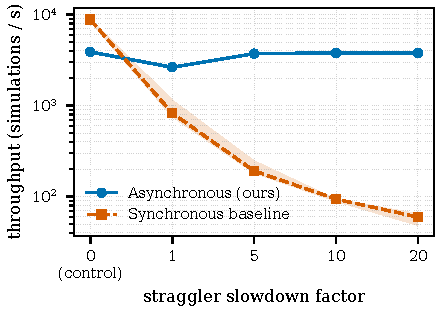
\includegraphics[width=0.6\linewidth]{figures/fig_straggler_throughput.pdf}
\caption{Throughput (median $+$ inter-quartile range over five replicates) versus straggler slowdown factor, including a $0\times$ no-straggler control. One worker carries a permanent post-evaluation delay of $0.1$\,s scaled by the factor. The synchronous baseline degrades sharply at the generation barrier (from ${\approx}8800$ sims/s at the control to ${\approx}60$ at $20\times$); the asynchronous method is robust (median ${\approx}2600$--$3900$ across the range, with no collapse). Note the logarithmic throughput axis.}\label{fig:straggler}
\end{figure}

\paragraph{Runtime heterogeneity.} Under stochastic log-normal runtime noise the asynchronous method sustains higher utilization (lower idle fraction) than the synchronous baseline, which idles at generation barriers (Fig.~\ref{fig:hetero}). Crucially, this utilization converts directly into inference quality: at a fixed wall-clock budget the synchronous baseline completes fewer and fewer simulations as the runtime spread $\sigma$ grows (it idles at every barrier) and its posterior-mean error to the analytic Gaussian posterior climbs several-fold (from ${\approx}0.05$ to ${\approx}0.28$), whereas the asynchronous method completes several-fold more simulations and holds its error essentially flat (${\approx}0.007$--$0.011$) (Fig.~\ref{fig:hetero-quality}). Removing the barrier therefore preserves not just the simulation rate but the \emph{inference} delivered per unit wall-clock.

\begin{figure}[t]
\centering
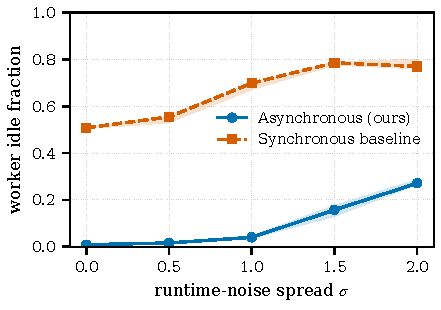
\includegraphics[width=0.6\linewidth]{figures/fig_hetero_idle.pdf}
\caption{Worker utilization loss under runtime heterogeneity: the fraction of worker wall-clock spent idle versus the runtime-noise spread $\sigma$ (five replicates; bands are inter-quartile ranges). The synchronous baseline idles at generation barriers (its idle fraction rises from ${\approx}0.51$ to ${\approx}0.79$ as heterogeneity grows) while the asynchronous method stays near-fully utilized (idle fraction ${\approx}0.01$ rising to ${\approx}0.27$).}\label{fig:hetero}
\end{figure}

\begin{figure}[t]
\centering
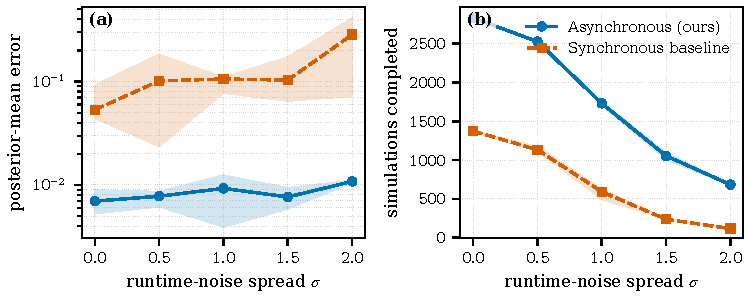
\includegraphics[width=\linewidth]{figures/fig_hetero_quality.pdf}
\caption{Inferential efficiency under runtime heterogeneity (Gaussian-mean benchmark, analytic posterior, fixed $60$\,s budget, five replicates; bands are inter-quartile ranges). Left: posterior-mean error to the analytic posterior versus runtime-noise spread $\sigma$; the synchronous baseline degrades sharply while the asynchronous method stays flat. Right: simulations completed within the budget; the synchronous baseline is starved by barrier idling as $\sigma$ grows, whereas the asynchronous method sustains several-fold higher completion.}\label{fig:hetero-quality}
\end{figure}

\paragraph{Parameter-coupled runtime (every-particle bias).} The study above slows simulations independently of their parameters; a sharper test couples runtime \emph{to the inferred parameter}, directly probing the every-particle bias of Limitation~(iv). On the Gaussian-mean benchmark ($48$ workers, $60$\,s budget, five replicates) we set the post-evaluation delay to $d(\mu)=\min\!\big(d_0\,e^{\,c(\mu-\mu_c)/\ell},\,d_{\max}\big)$ with base $d_0=0.02$\,s, centre $\mu_c=0$, length scale $\ell=0.15$, and cap $d_{\max}=0.5$\,s, and sweep the coupling strength $c\in\{0,0.5,1,2\}$ ($c=0$ recovers uniform runtime). Larger $c$ makes one region of parameter space evaluate far faster than its mirror image, so the asynchronous ``keep every accepted particle'' rule over-represents the fast region in the raw archive. The coupling has the intended effect: aggregate throughput falls as it steepens, by ${\approx}40\%$ for the asynchronous method (${\approx}1880 \to 1150$ sims/s) and more steeply for the barrier-bound baseline (${\approx}840 \to 250$; Fig.~\ref{fig:param-bias}a), confirming that the fast region dominates the raw sample counts. Yet the asynchronous posterior-mean error to the analytic Gaussian posterior does not increase as the coupling steepens; it stays ${\approx}0.01$ and comparable to the discard-latecomers synchronous baseline (Fig.~\ref{fig:param-bias}b). At the coupling levels tested the over-representation is measurable in the raw sampling rate but does not measurably distort the reported (unweighted top-$k$) posterior mean. A targeted ablation that removes the AMIS proposal adaptation ($S{=}0$) and re-runs the same coupling sweep leaves this robustness essentially unchanged --- the asynchronous posterior-mean error stays ${\approx}0.005$--$0.013$ with or without AMIS and shows no trend in the coupling --- which indicates that the raw archive is itself robust at these levels rather than that AMIS actively corrects the over-representation. Two finer tests that Limitation~(iv) motivates sharpen this rather than leave it open. First, we score the AMIS-\emph{reweighted} posterior --- the estimator the guarantees of \S\ref{sec:theory} concern, resampling the archive by the retroactive weight \eqref{eq:posterior-estimator} --- instead of the unweighted archive, and compare it against the no-AMIS variant ($S{=}0$) across the coupling sweep and a steeper regime (base delay $0.5$\,s, cap $8$\,s). The reweighted posterior recovers the analytic mean as accurately as the unweighted archive (absolute error ${\le}0.025$, no trend in the coupling) in both regimes and with or without AMIS; the reweighting's effect surfaces in the posterior \emph{spread}, not the mean --- it lowers the effective sample size (ESS fraction ${\approx}0.88$, vs ${\approx}0.99$ without AMIS), roughly triples the maximum normalised weight (${\approx}0.03$ vs ${\approx}0.01$), and widens the central $90\%$ interval by ${\approx}15\%$ --- so AMIS reshapes the tails but neither creates nor removes a mean bias at these coupling levels. Second, a drain-after-deadline variant lets every in-flight simulation finish past the wall-clock deadline and recomputes the posterior; comparing it against the censored run isolates the completion-time censoring that dividing by the proposal density does not correct. Draining moves the weighted posterior mean by at most $0.013$ --- comparable to the replicate-to-replicate spread (${\approx}0.01$) --- with no systematic direction, in both the mild and the steep regime. At these coupling levels the deadline censoring is therefore present in principle but negligible in effect, consistent with the sampler concentrating in the fast region near the posterior where few simulations are in flight at the deadline. We accordingly report the raw archive as robust here rather than claiming AMIS corrects the over-representation, and treat a formal censoring correction as future work (Limitation~(iv)).

\begin{figure}[t]
\centering
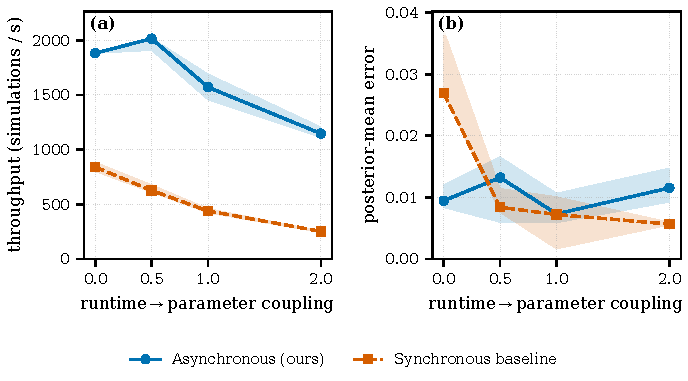
\includegraphics[width=0.92\linewidth]{figures/fig_param_bias.pdf}
\caption{Parameter-coupled runtime on the Gaussian-mean benchmark (analytic posterior; $48$ workers, $60$\,s budget, five replicates; bands are inter-quartile ranges). The post-evaluation delay grows with the inferred mean, so one region of parameter space is sampled far more often than its mirror image. (a) Aggregate throughput falls as the coupling steepens (more steeply for the barrier-bound baseline), confirming that the fast region dominates the raw sample counts. (b) Posterior-mean error to the analytic posterior nonetheless does not increase with coupling and stays comparable between the asynchronous method and the discard-latecomers synchronous baseline, so the over-representation does not measurably distort the reported posterior at these coupling levels.}\label{fig:param-bias}
\end{figure}

\paragraph{Strong scaling.} Lotka--Volterra is deliberately an \emph{adversarial} simulator for a scaling study: each evaluation takes only $\approx 2$\,ms, so the simulator occupies only a small fraction of each worker's wall-clock and there is essentially no per-evaluation compute to distribute. A dedicated instrumented run measures this productive fraction directly (Fig.~\ref{fig:lv-timing}): at the $48$-worker throughput peak a worker spends only ${\approx}25\%$ of its time inside the simulator, leaving ${\approx}75\%$ for coordination and idle waiting, and that productive share falls to ${\approx}8\%$ and then ${\approx}2\%$ as the job spreads from one node to three to six. The mechanism is the method's single shared population: every completed evaluation is broadcast to all workers so that each can propose from the current archive, an all-to-all exchange whose per-arrival cost grows with the worker count. On a near-instantaneous simulator this exchange saturates and then actively slows the productive ranks. Aggregate throughput therefore rises almost linearly while the job fits on one node ($149\to369\to1983\to6240$ sims/s at $1\to4\to16\to48$ workers) and then \emph{declines} across fully packed multi-node jobs (worker counts that are exact multiples of $48$): $6240\to4195\to2615\to2088\to1729$ sims/s at $48\to144\to192\to240\to288$ workers, i.e.\ $1\to3\to4\to5\to6$ nodes, because adding ranks beyond one node lengthens the all-to-all exchange faster than it adds useful work. This is a property of coordinating a near-instantaneous simulator across a single shared population, not of asynchrony as such (precisely the regime in which asynchrony has least to offer), and it lifts once the simulator carries real per-evaluation cost that amortizes the coordination (the Cellular Potts result of \S\ref{sec:results-cpm}; Fig.~\ref{fig:scaling}, right). To keep the comparison fair at high core counts we give the synchronous ABC-SMC baseline a \emph{population size equal to the worker count} (a smaller population cannot occupy every core); it then uses all allocated cores and scales steadily, from ${\approx}440$ sims/s at $16$ workers to ${\approx}6000$ at $288$ (Table~\ref{tab:scaling}). On this free simulator the asynchronous method leads while the job stays within a few nodes (${\approx}4.5\times$ at $16$ workers, ${\approx}2\times$ at one full node), but its lead \emph{erodes} with scale and the fair synchronous baseline overtakes it beyond three nodes, where the growing all-to-all coordination cost dominates and the asynchronous method leaves most of the allocation idle. This is the honest boundary of the asynchronous advantage on a cheap, homogeneous simulator; it is largest exactly in the heterogeneous and straggler-prone regimes where barriers otherwise waste compute. The archive size sets where that boundary falls, because the per-arrival proposal reconstruction is $\mathcal{O}(k)$: enlarging the archive tenfold to $k=1000$ costs throughput at every worker count --- $39\%$ at the single-node peak ($6240\to3804$ sims/s) --- and brings the crossover with the fair baseline in from beyond three nodes to a single node (Table~\ref{tab:scaling}). Sweeping $k$ across $\{50,100,200,400,800,1000\}$ at every worker count resolves that cost into a smooth monotone decline in throughput and a single step in the crossover, which moves in from beyond three nodes to three nodes at $k\ge400$ (Table~\ref{tab:k-frontier}). The archive size is therefore a systems cost as well as a statistical knob --- but, put on the same axis as the calibration it buys, the two turn out \emph{not} to trade off over this range: the best-calibrated archive is also within $7\%$ of the fastest, and every archive larger than $k=100$ is both slower and worse calibrated (\S\ref{sec:results-validity}, Table~\ref{tab:k-frontier}).

\begin{table}[t]
\caption{Strong scaling on Lotka--Volterra: median simulation throughput (sims/s) at a 180\,s budget, over five replicates (Fig.~\ref{fig:scaling}, left, shows the inter-quartile spread). Asynchronous (ours) at both archive sizes vs.\ synchronous baseline. Multi-node points use \emph{fully packed} nodes (worker counts that are exact multiples of $48$); at counts above $100$ the synchronous baseline is given \emph{population size equal to the worker count} so it can occupy every core (a population of $100$ leaves the surplus idle), which is why it keeps scaling here. The asynchronous method peaks on one node and then declines as multi-node coordination dominates, so the baseline overtakes it beyond three nodes at $k=100$. Enlarging the archive tenfold costs throughput at every scale --- the per-arrival proposal reconstruction is $\mathcal{O}(k)$ --- and moves that crossover in to a single node.}\label{tab:scaling}
\centering
\begin{tabular}{@{}lcccccccc@{}}
\toprule
Workers & 1 & 4 & 16 & 48 & 144 & 192 & 240 & 288 \\
Nodes & $<$1 & $<$1 & $<$1 & 1 & 3 & 4 & 5 & 6 \\
\midrule
Synchronous & 105 & 96 & 437 & 2952 & 3757 & 4322 & 4539 & 6034 \\
Asynchronous ($k=100$) & 149 & 369 & 1983 & 6240 & 4195 & 2615 & 2088 & 1729 \\
Asynchronous ($k=1000$) & 106 & 133 & 620 & 3804 & 2804 & 1957 & 1587 & 1336 \\
\botrule
\end{tabular}
\end{table}

\begin{figure}[t]
\centering
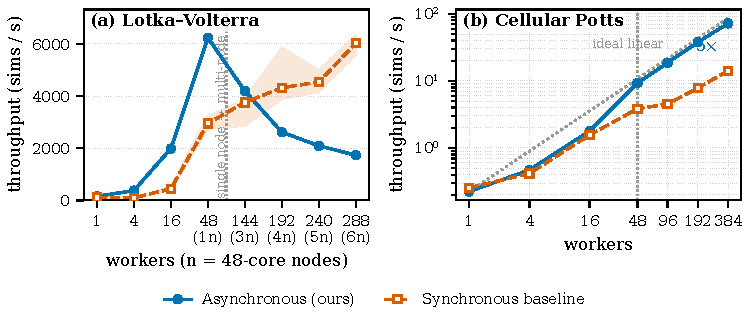
\includegraphics[width=\linewidth]{figures/fig_scaling_combined.pdf}
\caption{Strong scaling: median simulation throughput versus worker count at a fixed wall-clock budget, asynchronous (ours) vs.\ a synchronous baseline given \emph{population size equal to the worker count} so it can occupy every core. \textbf{Left:} Lotka--Volterra (near-instant simulator, $\approx 2$\,ms/eval; $180$\,s budget; categorical $x$-axis; bands are inter-quartile ranges over five replicates; node count $n$ in labels). With no per-evaluation compute to distribute, the asynchronous method's single-population all-to-all coordination cost grows with the worker count: throughput rises within one node, peaks there, and then declines across multi-node jobs, so its lead over the fair, steadily scaling baseline erodes and the baseline overtakes it beyond three nodes. \textbf{Right:} Cellular Potts (costly \texttt{cellsInSilico} simulator; $1800$\,s budget; log--log; medians over replicates). Real per-evaluation cost amortizes the coordination, so the asynchronous method tracks ideal-linear scaling (dotted) to eight nodes ($384$ workers, ${\approx}97\%$ parallel efficiency) while the barrier-bound baseline scales only sub-linearly, a ${\approx}5\times$ gap at $384$ workers that \emph{grows} with scale.}\label{fig:scaling}
\end{figure}

\begin{figure}[t]
\centering
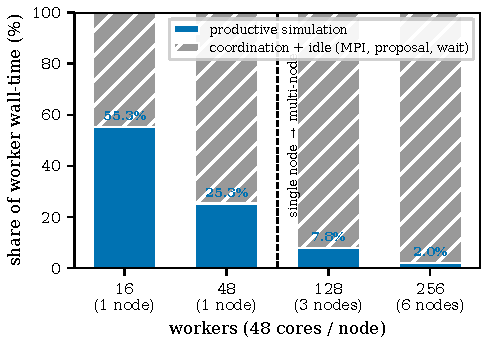
\includegraphics[width=0.66\linewidth]{figures/fig_lv_timing.pdf}
\caption{Measured decomposition of asynchronous worker wall-time on Lotka--Volterra ($k=100$; $180$\,s budget) from a dedicated instrumented run. The productive simulation fraction (blue, annotated) --- the share of worker wall-clock spent inside the simulator --- collapses from $55\%$ at $16$ workers to $2\%$ at $256$, while coordination and idle (MPI exchange, per-arrival proposal reconstruction, serialization, waiting) dominate exactly as the job spreads beyond one node (16/48 = 1 node; 128 = 3 nodes; 256 = 6 nodes). The strong-scaling decline of Fig.~\ref{fig:scaling} is therefore a measured property of coordinating a near-instantaneous simulator, not an inferred one.}\label{fig:lv-timing}
\end{figure}

\subsection{Posterior validity (RQ1)}\label{sec:results-validity}
Having established the systems advantage, we ask what it costs in inference quality. Across calibration and matched-budget posterior recovery the reported streaming posterior --- the full-history AMIS estimator \eqref{eq:posterior-estimator} --- is comparable to the matched synchronous baseline in low dimensions and under multimodality, and in four dimensions errs toward conservatism (it mildly over-covers) rather than over-confidence.

\paragraph{Calibration.} Table~\ref{tab:sbc} reports SBC empirical coverage on the Gaussian-mean model (1000 trials, matched simulation budget), for the reported full-history AMIS posterior. The asynchronous method tracks the nominal level closely ($0.51/0.80/0.90/0.94$ at the $0.50/0.80/0.90/0.95$ levels), within Monte Carlo error of nominal at every level; the synchronous baseline under-covers at every level ($0.35/0.63/0.75/0.83$), i.e.\ it is over-confident. At 1000 trials a coverage estimate carries a Monte Carlo standard error of only ${\approx}\,\pm0.007$--$0.016$, well below the ${\approx}0.12$--$0.17$ gap between the methods, so the ordering is resolvable rather than noise: on this benchmark the streaming estimator is \emph{better} calibrated than the matched synchronous baseline. Reporting the estimator over the full evaluated history rather than the top-$k$ archive alone matters even here: in a paired $500$-trial run that changes only the reported support, the truncated archive mildly under-covers at the top levels ($0.89/0.92$ at the $0.90/0.95$ levels), which the full-history report corrects to nominal --- a reporting-support effect that grows with dimension, as the multimodal and four-dimensional tests below make explicit. This test is on a one-dimensional model with an analytic posterior; the higher-dimensional and multimodal settings where the archive/proposal approximations are most likely to bite are probed separately below. Figure~\ref{fig:sbc} shows the corresponding coverage curve and rank histogram.

\paragraph{Calibration under multimodality and in higher dimensions.} To probe exactly those settings, we run SBC (1000 trials, matched simulation budget) on two harder targets, reporting the same full-history AMIS posterior. The first is a \emph{multimodal} model $y_i\sim\mathcal N(\theta^2,\sigma^2)$: the sign ambiguity gives a symmetric bimodal posterior at $\pm\sqrt{\bar y}$, the case a top-$k$ archive is most at risk of collapsing onto a single mode. It does not collapse --- the archive retains \emph{both} modes in $85.7\%$ of trials and the mode containing the true value in $86.7\%$ (the remainder are largely near-$\theta{=}0$ trials where the two modes merge), the importance weights stay near-uniform (median effective-sample-size fraction $0.99$, median maximum normalised weight $0.011$), and coverage tracks the nominal level ($0.50/0.82/0.91/0.96$), calibrated within Monte Carlo error. The second is the \emph{four-dimensional} g-and-k model, where the reporting-support choice bites. The reported full-history posterior is \emph{conservative}: it mildly over-covers at every level and parameter (e.g.\ empirical coverage $0.62/0.91/0.96/0.99$ at the $0.50/0.80/0.90/0.95$ levels for the location parameter $A$, and similarly for $B,g,k$), because the finite-$\epsilon$ smooth-ABC posterior it reports is over-dispersed at the loose bandwidth a four-dimensional budget reaches. The efficient top-$k$ archive used for online proposal sits at the opposite end: it is over-concentrated and would instead \emph{under}-cover ($0.85/0.89$ at the $0.90/0.95$ levels for $A$), with healthy weights throughout (median effective-sample-size fraction $0.81$), so the miscalibration is a reporting-support effect, not weight degeneracy. The calibrated posterior is therefore \emph{bracketed} between the over-concentrated archive core and the over-dispersed full history, and the amount of history reported is the dispersion knob: widening the reported support from the archive toward the full history raises coverage monotonically and continuously through nominal --- for $A$, $0.85/0.89 \to 0.93/0.96 \to 0.95/0.98 \to 0.97/0.99$ at the $0.90/0.95$ levels for reported sizes $M=200/500/1500/\text{full}$, crossing nominal near $M\approx400$--$800$ (the shape parameters $B$ and $k$ are already near-nominal at $M{=}500$, e.g.\ $0.89/0.94$ for $B$). This is a property of \emph{how much of the history is reported}, not of the AMIS weighting (whose importance weights stay well-conditioned) or of the budget: doubling the simulation budget to $80{,}000$ per trial leaves the archive coverage essentially unchanged ($0.85/0.89$ at the $0.90/0.95$ levels for $A$, within Monte Carlo error for $B,g,k$). We accordingly report the streaming estimator, evaluated over the full evaluated history, as well calibrated in one dimension and under multimodality, and conservative --- over-covering rather than over-confident --- in four dimensions; an intermediate reported support ($M\approx400$--$800$), a larger archive, or the defensive-mixture floor (\S\ref{sec:limitations}) tighten the four-dimensional report toward exactly nominal.

\paragraph{How calibration depends on the archive size and the snapshot buffer.} The tests above fix $k$ and $S$ per benchmark, which leaves open whether the two efficiency knobs must be retuned as the dimension grows. To settle this we sweep them directly on a $d$-dimensional Gaussian-mean target, $y_i\sim\mathcal N(\theta,\sigma^2 I_d)$ with $\theta\in\mathbb R^d$ under a flat box prior, whose posterior is known exactly at every $d$ (SBC against that exact posterior returns $0.496/0.794/0.905/0.952$, confirming the target itself is calibrated, so any departure below is a property of the method). The grid is $d\in\{1,2,4,8,16\}\times k\in\{50,100,200,400,800\}\times S\in\{0,5,20,50\}$, $1000$ trials per cell, reporting the same full-history estimator (Table~\ref{tab:ks-sweep}).

The two knobs behave quite differently. The snapshot buffer $S$ has a threshold and then saturates: at $S=0$ the estimator is over-confident in low dimensions (mean deviation $-0.088$ at $d=1,2$), $S=5$ removes essentially all of it ($-0.001$), and $S=20$ and $S=50$ add nothing further --- at any dimension. The value of a richer balance-heuristic denominator therefore does \emph{not} grow with $d$ over this range, and the fixed $S=20$ we use throughout sits comfortably above the knee. The archive size $k$ is the opposite: its effect is large, strongly dimension-dependent, and \emph{not} monotone. Small archives can be severely over-confident in intermediate dimensions --- at $d=8,k=50$ empirical coverage is $0.29/0.52/0.63/0.71$ against the nominal $0.50/0.80/0.90/0.95$, a failure that persists at every $S$ --- while intermediate archives over-cover in the same regime ($+0.18$ to $+0.20$ at $k=200$--$400$). We note that this does not follow the floor a naive count of covariance parameters would predict: the perturbation covariance is a full $d\times d$ matrix estimated from the archive, suggesting $k\gtrsim d(d{+}1)/2$, yet $d=8$ fails at $k=50>36$ while $d=16$ remains within $0.06$ of nominal at $k=50<136$. The reading this supports is that $d=16$ is protected by its own difficulty: with $20{,}000$ simulations over a $[-5,5]^{16}$ prior the sampler barely concentrates, so the reported posterior stays broad and covers almost by default, whereas $d=8$ has enough signal to concentrate but not enough to concentrate correctly. Two further runs test that reading rather than leaving it as narrative. First, it predicts that a \emph{higher} dimension should look benign again: at $d=32$ the coverage is $0.55$--$0.57$, $0.83$--$0.84$, $0.92$, $0.96$ at the four levels for every $k\in\{50,100,800\}$ --- mildly conservative and nowhere near the $d=8$ failure, even at $k=50$. Second, the failure is not a budget shortfall: doubling the simulation budget at $d=8,k=50$ makes coverage slightly \emph{worse} ($0.26/0.47/0.58/0.67$ against $0.29/0.52/0.63/0.71$ at the original budget), exactly as expected if the extra simulations sharpen an already mislocated posterior rather than repairing it. We therefore do not offer a closed-form rule for $k$; the practical guidance is that the archive size is the dispersion knob (\S\ref{sec:results-validity}), that its safe range is problem- and dimension-specific, and that it should be chosen by checking calibration directly rather than by a formula.

\paragraph{The archive size does not, in this range, trade calibration against throughput.} Because $k$ has both a statistical effect (above) and a systems cost --- per-arrival proposal reconstruction is $\mathcal{O}(k)$, so a larger archive is slower at every worker count (\S\ref{sec:results-hpc}) --- it is natural to expect the two to pull against each other, and to have to buy calibration with throughput. Measuring both on one axis shows that expectation is wrong over the range we can test. Table~\ref{tab:k-frontier} puts the throughput cost of $k$ next to its worst-case miscalibration over the dimensions swept, using a throughput grid matched on everything but $k$ (Lotka--Volterra, $180$\,s wall cap, five replicates, worker counts $1$--$288$: $k\in\{100,1000\}$ from the main scaling run and $k\in\{50,200,400,800\}$ from a dedicated $k$-frontier run sharing that configuration). Of the six archive sizes, only two are Pareto-optimal, and they are the two smallest: $k=100$ is simultaneously the best-calibrated setting tested (worst deviation $0.064$, at $d=4$) and within $7\%$ of the fastest ($6240$ vs $6684$ simulations/s at the single-node peak). Every larger archive is dominated by it on \emph{both} axes at once --- $k=200$ is $5\%$ slower and nearly three times worse calibrated ($0.180$), $k=400$ is $14\%$ slower and $0.195$, and $k=800$ costs $31\%$ of throughput to end up still slightly worse calibrated than $k=100$ ($0.074$). The only genuinely faster archive, $k=50$, is the catastrophic one ($0.250$ at $d=8$). So the practical shape of the $k$ decision is not a frontier to negotiate but a floor to clear: go far enough above the small-archive failure region, and then stop, because further enlargement buys no calibration and costs throughput monotonically.

Two qualifications keep this from being read too broadly. The join is on $k$ alone and the two axes come from different benchmarks by design --- calibration needs a target whose posterior is known at every $d$, throughput needs the regime where an $\mathcal{O}(k)$ per-arrival cost is most exposed. That second choice makes the throughput column an \emph{upper} bound on the relative cost of $k$: Lotka--Volterra evaluations take ${\approx}2$\,ms, so coordination dominates there, and on a cost-bearing simulator the per-evaluation work amortizes the archive operation (\S\ref{sec:results-cpm}). The conclusion is therefore conservative in the right direction --- even where $k$ is most expensive, the best-calibrated archive is nearly free. What $k$ \emph{does} change at scale is where the fair synchronous baseline overtakes the asynchronous method, and there it acts as a step rather than a smooth trade: the crossover sits beyond three fully packed nodes for $k\le200$ and moves in to three nodes for $k\ge400$ (last column).

\begin{table}[t]
\caption{Calibration sensitivity to the archive size $k$ and the AMIS snapshot buffer $S$ on the $d$-dimensional Gaussian-mean target ($1000$ trials per cell; entries are the mean signed deviation of empirical from nominal coverage over the $0.50/0.80/0.90/0.95$ levels and the $d$ parameters). Negative is over-confident, positive is conservative; $0.000$ is exactly calibrated. \textbf{Left:} varying $k$ at $S=20$. \textbf{Right:} varying $S$ at $k=100$.}\label{tab:ks-sweep}
\centering
\begin{tabular}{@{}lccccc@{}}
\toprule
& \multicolumn{5}{c@{}}{archive size $k$ (at $S=20$)} \\
\cmidrule(l){2-6}
& 50 & 100 & 200 & 400 & 800 \\
\midrule
$d=1$  & -0.014 & -0.003 & +0.006 & +0.006 & +0.074 \\
$d=2$  & -0.020 & -0.006 & +0.009 & +0.030 & +0.072 \\
$d=4$  & +0.025 & +0.064 & +0.094 & +0.133 & +0.063 \\
$d=8$  & \textbf{-0.250} & +0.055 & +0.180 & +0.195 & +0.061 \\
$d=16$ & -0.047 & +0.028 & +0.049 & +0.053 & +0.055 \\
\botrule
\end{tabular}
\vspace{0.6em}

\begin{tabular}{@{}lcccc@{}}
\toprule
& \multicolumn{4}{c@{}}{snapshot buffer $S$ (at $k=100$)} \\
\cmidrule(l){2-5}
& 0 & 5 & 20 & 50 \\
\midrule
$d=1$  & \textbf{-0.088} & -0.001 & -0.003 & -0.005 \\
$d=2$  & \textbf{-0.088} & -0.001 & -0.006 & -0.003 \\
$d=4$  & +0.039 & +0.068 & +0.064 & +0.064 \\
$d=8$  & +0.065 & +0.006 & +0.055 & +0.074 \\
$d=16$ & -0.010 & +0.010 & +0.028 & +0.034 \\
\botrule
\end{tabular}
\end{table}

\begin{table}[t]
\caption{The archive size on both of its axes at once. \textbf{Throughput}: median asynchronous throughput at the single-node peak ($48$ workers) on Lotka--Volterra, $180$\,s wall cap, five replicates ($k\in\{100,1000\}$ from the main scaling run, $k\in\{50,200,400,800\}$ from the matched $k$-frontier run), and its change relative to the $k{=}100$ we use throughout. \textbf{Calibration}: worst absolute deviation of empirical from nominal coverage over the dimensions of the $d$-dimensional Gaussian-mean sweep at $S{=}20$ (Table~\ref{tab:ks-sweep}), with the dimension attaining it. \textbf{Crossover}: fully packed nodes at which the fair synchronous baseline (population $=$ worker count) overtakes the asynchronous arm. Only $k{=}50$ and $k{=}100$ are Pareto-optimal; every larger archive is both slower \emph{and} worse calibrated than $k{=}100$. The sweep did not include $k{=}1000$.}\label{tab:k-frontier}
\centering
\begin{tabular}{@{}lccccc@{}}
\toprule
$k$ & sims/s at $W{=}48$ & vs.\ $k{=}100$ & worst $|\Delta\text{cov}|$ & at & baseline overtakes \\
\midrule
50   & 6684 & $+7\%$  & \textbf{0.250} & $d{=}8$ & beyond 3 nodes \\
100  & 6240 & ---     & \textbf{0.064} & $d{=}4$ & beyond 3 nodes \\
200  & 5904 & $-5\%$  & 0.180 & $d{=}8$ & beyond 3 nodes \\
400  & 5393 & $-14\%$ & 0.195 & $d{=}8$ & 3 nodes \\
800  & 4331 & $-31\%$ & 0.074 & $d{=}1$ & 3 nodes \\
1000 & 3804 & $-39\%$ & ---   & ---     & 3 nodes \\
\botrule
\end{tabular}
\end{table}

\begin{table}[t]
\caption{SBC empirical coverage on Gaussian-mean inference (parameter $\mu$, 1000 trials; Monte Carlo standard error ${\approx}\,\pm0.007$--$0.016$), for the reported full-history AMIS posterior. Closer to the nominal level is better.}\label{tab:sbc}
\centering
\begin{tabular}{@{}lcccc@{}}
\toprule
Method & 0.50 & 0.80 & 0.90 & 0.95 \\
\midrule
Synchronous baseline & 0.35 & 0.63 & 0.75 & 0.83 \\
Asynchronous (ours) & 0.51 & 0.80 & 0.90 & 0.94 \\
\botrule
\end{tabular}
\end{table}

\begin{figure}[t]
\centering
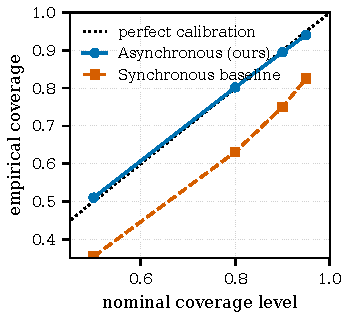
\includegraphics[width=0.48\linewidth]{figures/fig_sbc_coverage.pdf}\hfill
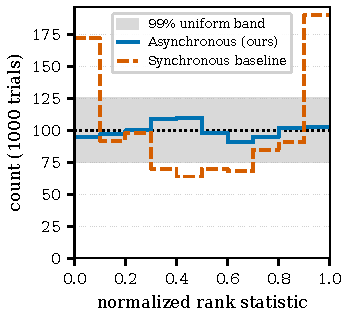
\includegraphics[width=0.48\linewidth]{figures/fig_sbc_rank.pdf}
\caption{Simulation-based calibration on Gaussian-mean inference (1000 trials; the reported full-history AMIS posterior): empirical coverage versus nominal level (left) and rank histogram (right). The asynchronous estimator is close to calibrated.}\label{fig:sbc}
\end{figure}

\paragraph{Posterior recovery.} On g-and-k the asynchronous method reaches a slightly \emph{lower} Wasserstein distance to the truth than the synchronous baseline at matched wall-clock budget ($0.078$ vs.\ $0.090$, inter-quartile ranges $[0.077,0.083]$ and $[0.082,0.093]$), and on Lotka--Volterra the two are comparable with the asynchronous method marginally lower ($0.316$ vs.\ $0.332$, overlapping inter-quartile ranges). On the expensive Cellular Potts simulator the ordering reverses and the asynchronous method is \emph{modestly but consistently behind}: the async$-$sync difference is positive across $87.5\%$ of the budget, ending at ${+}0.043$ with an inter-quartile envelope of $[0.019,0.052]$ that excludes zero, and it never exceeds ${\approx}0.06$ against a Wasserstein scale of ${\approx}0.4$ (Figs.~\ref{fig:posterior-recovery}c and~\ref{fig:cpm-diff}). One property of this benchmark bounds how that gap should be read: the Wasserstein-to-reference \emph{rises} with compute for both methods (asynchronous $0.37\to0.48$), because the Cellular Potts parameters are only weakly identified (\S\ref{sec:results-cpm}) and the comparison is against a reference point rather than a known posterior, so a diffuse cloud scores better than a posterior that has concentrated slightly off that reference. The metric therefore penalizes concentration on this target, and the asynchronous method --- which completes ${\approx}2\times$ the evaluations in the same budget --- concentrates fastest. Per-parameter posteriors and joint marginals are consistent with the known/reference values. In the straggler runs (which compute posterior quality) the final Wasserstein distances are comparable between methods (asynchronous $\approx0.07$--$0.08$ vs.\ synchronous $\approx0.07$). On the Gaussian-mean benchmark, which has a closed-form posterior, the asynchronous method recovers the posterior mean to within $\approx0.002$--$0.038$ absolute error (comparable to the synchronous baseline, $\approx0.006$--$0.021$, and far tighter than a rejection-ABC reference) and tracks the baseline's Wasserstein-vs-time trajectory throughout the budget (Fig.~\ref{fig:gaussian-recovery}); the SBC calibration above is unaffected.

\begin{figure}[t]
\centering
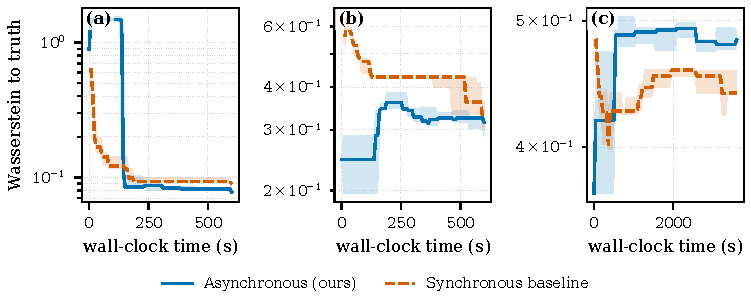
\includegraphics[width=\linewidth]{figures/fig_posterior_recovery.pdf}
\caption{Posterior quality (Wasserstein distance to the truth/reference, lower is better) versus wall-clock time on g-and-k (left), Lotka--Volterra (middle), and Cellular Potts (right), asynchronous vs.\ synchronous; shaded bands are inter-quartile ranges over five replicates. On g-and-k the asynchronous method reaches a slightly lower Wasserstein distance within the budget, on Lotka--Volterra the two are comparable, and on Cellular Potts the asynchronous method is modestly but consistently behind. Note that on the weakly identified Cellular Potts target the distance-to-reference \emph{increases} with compute for both methods, so the metric penalizes the method that concentrates fastest (\S\ref{sec:results-validity}).}\label{fig:posterior-recovery}
\end{figure}

\begin{figure}[t]
\centering
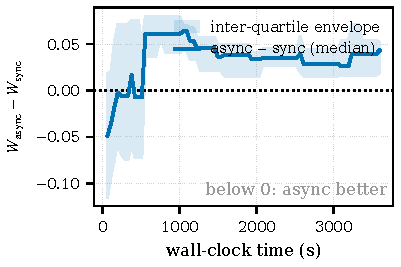
\includegraphics[width=0.55\linewidth]{figures/fig_cpm_recovery_diff.pdf}
\caption{Cellular Potts posterior-quality \emph{difference} (asynchronous minus synchronous Wasserstein to the reference) versus wall-clock time, with a zero reference line and an inter-quartile envelope over five replicates (the per-method Cellular Potts curves of Fig.~\ref{fig:posterior-recovery}c, differenced). The difference is positive --- asynchronous behind --- across $87.5\%$ of the budget, ending at ${+}0.043$ with an envelope of $[0.019,0.052]$ that excludes zero; it straddles zero only over the first ${\approx}510$\,s. The gap is nonetheless small in absolute terms, never exceeding ${\approx}0.06$ against an absolute Wasserstein of ${\approx}0.4$, and it is measured against a reference point on a weakly identified target whose distance-to-reference grows as either method concentrates (\S\ref{sec:results-validity}, \S\ref{sec:results-cpm}).}\label{fig:cpm-diff}
\end{figure}

\begin{figure}[t]
\centering
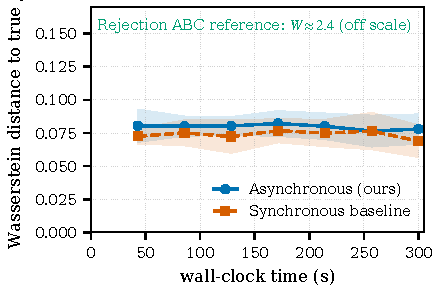
\includegraphics[width=0.6\linewidth]{figures/fig_gaussian_recovery.pdf}
\caption{Gaussian-mean posterior recovery: Wasserstein distance to the true $\mu$ versus wall-clock time, with replicate confidence bands. The asynchronous method (archive) tracks the matched synchronous baseline (generation) throughout the budget, both far below the annotated rejection-ABC reference ($W\approx2.4$).}\label{fig:gaussian-recovery}
\end{figure}

\subsection{Realistic simulator: Cellular Potts (RQ3)}\label{sec:results-cpm}
The Cellular Potts benchmark runs end-to-end with the real \texttt{cellsInSilico} simulator, a realistic, expensive, heterogeneous-runtime workload and the regime the method targets.

\paragraph{Strong scaling.} Because each Cellular Potts evaluation carries real cost, the per-arrival coordination that capped Lotka--Volterra is amortized, and the asynchronous method scales almost linearly all the way to eight nodes (Fig.~\ref{fig:scaling}, right): median throughput rises from $0.2$ to $72.0$ simulations/s over $1$ to $384$ workers and, unlike the near-instantaneous Lotka--Volterra case, keeps scaling \emph{across} the single-node$\to$multi-node boundary, each node-doubling roughly doubling throughput ($9.3\to18.7\to37.8\to72.0$ sims/s at $48\to96\to192\to384$ workers), for $\approx 97\%$ parallel efficiency relative to the single-node rate. The synchronous baseline, given a population equal to the worker count so it too can occupy every core, scales only \emph{sub-linearly} over the same range ($3.8\to4.5\to7.8\to14.2$ sims/s at $48\to96\to192\to384$ workers, ${\approx}50\%$ efficiency), so at $384$ workers the asynchronous method sustains ${\approx}5\times$ its throughput, a gap that \emph{widens} with scale. This is the regime the method is built for: an expensive, heterogeneous simulator where the generation barrier, not per-arrival overhead, is the binding cost. Worker utilization makes the mechanism explicit (Fig.~\ref{fig:cpm-util}): the asynchronous method keeps workers ${\approx}98.9$--$99.8\%$ busy across all scales, whereas the synchronous baseline, even with every core filled within a generation, then waits for the slowest simulation at the barrier, so its utilization falls to ${\approx}24$--$29\%$ ($41\%\to24\%\to26\%\to29\%$ from $48$ to $384$ workers, i.e.\ ${\approx}70$--$76\%$ idle at every multi-node scale). This barrier idle, not per-arrival overhead, is what holds the synchronous throughput to sub-linear scaling while the asynchronous method tracks the ideal. (We report medians throughout.)

\begin{figure}[t]
\centering
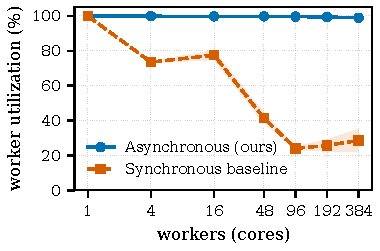
\includegraphics[width=0.52\linewidth]{figures/fig_cpm_util.pdf}
\caption{Cellular Potts worker utilization (fraction of worker wall-clock spent inside the simulator) versus worker count ($1800$\,s budget; error bars are $\pm1$ s.d.); the synchronous baseline uses a population equal to the worker count (Fig.~\ref{fig:scaling}, right). The asynchronous method stays ${\approx}98.9$--$99.8\%$ utilized at every scale, while the synchronous baseline, even filling every core within a generation, then idles at the barrier waiting for the slowest simulation, so its utilization falls to ${\approx}24$--$29\%$ ($41\%\to24\%\to26\%\to29\%$ at $48/96/192/384$ workers, i.e.\ ${\approx}70$--$76\%$ idle at every multi-node scale). This barrier idle is the measured mechanism behind the synchronous method's sub-linear scaling in Fig.~\ref{fig:scaling} (right).}\label{fig:cpm-util}
\end{figure}

\paragraph{The barrierized twin at this scale.} The twin comparison of \S\ref{sec:results-hpc} isolates synchronization on the two synthetic benchmarks; here we run it on the real simulator, at the same four worker counts and the same $k{=}100$, simulation-limited at $40$ evaluations per worker (Table~\ref{tab:twin-cpm}). Two things come out of it, and the second is the more interesting.

First, the barrier alone costs a factor that is remarkably \emph{stable} across scale: $1.9\times$ at one, two and four nodes, rising to $2.8\times$ at eight. The external pyABC baseline's penalty over the same range grows much faster, from $2.4\times$ to $5.1\times$. The twin is therefore consistently the faster of the two synchronous arms, and the distance between them widens with scale --- which is the honest answer to the question the twin was built to ask, and it is not the flattering one. On this workload the barrier is a \emph{major but not exclusive} cause of the cross-algorithm gap: it accounts for roughly half to three-quarters of it in log terms, and the residual, which grows with worker count, has to come from pyABC's other differences (its probabilistic-rejection step, its classical population weighting, and its own coordination costs) rather than from synchronization. We therefore do \emph{not} claim the Cellular Potts gap is attributable to the barrier alone --- only that the barrier is the single largest identified component of it. This is also the opposite ordering to the straggler and heterogeneity benchmarks, where the twin ran far \emph{slower} than pyABC because pyABC's latecomer discarding rescues it from waiting on the slowest draw; with no injected pathology, that rule has little to exploit and our more efficient propagator keeps the twin ahead.

Second --- and this is the more useful finding --- the barrier does not merely reduce throughput, it makes throughput \emph{unpredictable}. The asynchronous arm's five replicates agree to within $1.3\%$ at every scale (coefficient of variation $0.6$--$1.3\%$), while the twin's spread across the \emph{same} seeds is $25$--$54\%$: at $48$ workers its replicates run at $1.7$, $2.1$, $4.9$, $5.9$ and $6.0$ simulations/s, a factor of $3.5$ between fastest and slowest. The mechanism is the one the utilization measurement already shows: a generation ends only when its slowest evaluation does, so the whole job inherits the cost of the most expensive parameter draw in each generation, and on this benchmark simulation cost varies strongly with the parameters. Asynchrony removes that coupling --- a slow draw delays only its own worker --- which is why the asynchronous arm's throughput is reproducible to within a percent while its barrierized twin, running identical proposals from identical seeds, varies by more than threefold. For a practitioner this is arguably the more consequential of the two effects: a median slowdown can be budgeted for, a factor-of-three variance in time-to-result cannot.

One note on the twin as an instrument. It intermittently deadlocks at $\ge192$ ranks --- we observed five hangs while collecting this table, one in the MPI teardown and the others mid-run --- so individual replicates had to be retried. Every combination did complete, and all twenty entries here are full runs; but the twin is a diagnostic built for this comparison rather than a robust implementation, and at these rank counts it needs supervision.

\begin{table}[t]
\caption{Barrierized twin on the Cellular Potts workload: median throughput (simulations/s) over five replicates, $k{=}100$, simulation-limited at $40$ evaluations per worker. CV is the coefficient of variation across replicates. The barrier's own cost is nearly flat from one to four nodes ($1.9\times$) and rises to $2.8\times$ at eight, while the external pyABC baseline's penalty grows from $2.4\times$ to $5.1\times$ over the same range --- so the barrier is the single largest identified component of the cross-algorithm gap but not the whole of it, and the residual grows with scale. The second row-pair is the more useful finding: the twin's replicate spread is $25$--$54\%$ against the asynchronous arm's $0.6$--$1.3\%$ on the same seeds, because a generation inherits the cost of its most expensive parameter draw. Synchronization makes throughput unpredictable as well as lower. The pyABC baseline has three replicates at $192$ and $384$ workers (its fair population$=W$ shards); all twin and asynchronous entries have five.}\label{tab:twin-cpm}
\centering
\begin{tabular}{@{}lcccc@{}}
\toprule
Workers ($=$ cores) & 48 (1 node) & 96 (2) & 192 (4) & 384 (8) \\
\midrule
Asynchronous (ours)     & 9.33 & 18.67 & 37.75 & 71.98 \\
\quad CV                & $0.9\%$ & $1.3\%$ & $0.6\%$ & $1.3\%$ \\
Barrierized twin        & 4.87 & 10.00 & 20.24 & 25.54 \\
\quad CV                & $50.7\%$ & $53.8\%$ & $24.8\%$ & $49.8\%$ \\
Synchronous pyABC baseline & 3.85 & 4.53 & 7.85 & 14.17 \\
\midrule
Ratio, twin             & $1.9\times$ & $1.9\times$ & $1.9\times$ & $2.8\times$ \\
Ratio, pyABC baseline   & $2.4\times$ & $4.1\times$ & $4.8\times$ & $5.1\times$ \\
\botrule
\end{tabular}
\end{table}

\paragraph{Posterior quality.} On the inference side the asynchronous method produces marginals of similar shape to the synchronous baseline (Fig.~\ref{fig:cpm-posterior}), though it trails modestly on distance-to-reference (\S\ref{sec:results-validity}): the cell-motility parameter concentrates near its reference value, while the division rate is only weakly identified (for \emph{all} methods, the baseline included). This weak identification is a structural property of the inference problem, not of asynchrony: at this scale the division-rate and motility parameters are near-degenerate (both chiefly modulate the cell count that the summaries resolve), so neither method separates them and both improve only modestly on rejection ABC. The matched comparison therefore isolates the systems advantage as largely \emph{orthogonal} to identifiability: both methods are limited chiefly by the problem. On the summary metric the asynchronous method is modestly behind over the full budget (${+}0.043$ in Wasserstein-to-reference against a scale of ${\approx}0.4$; \S\ref{sec:results-validity}), so we report its throughput advantage as bought at a small quality cost on this benchmark rather than at none --- with the caveat that the metric rewards dispersion on a weakly identified target, and that the asynchronous method, concentrating fastest, is the one it penalizes most. Establishing the same quality with a synchronous matched baseline at the still larger scales the method targets would itself be prohibitively wasteful, precisely the cost the barrier-free design removes.

\begin{figure}[t]
\centering
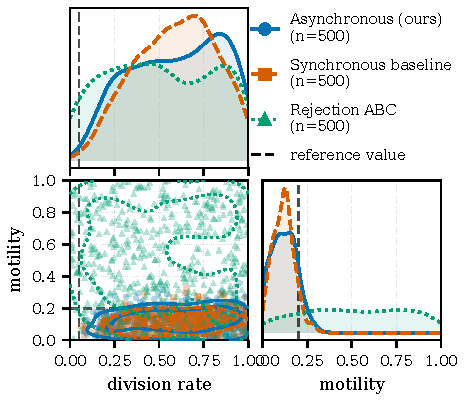
\includegraphics[width=0.62\linewidth]{figures/fig_cpm_corner.pdf}
\caption{Cellular Potts posterior (division rate, motility) on the real \texttt{cellsInSilico} simulator: asynchronous (blue), synchronous baseline (red), and rejection ABC (green), with dashed lines at the reference values. The asynchronous posterior is drawn from its AMIS estimator ($500$ resampled draws); the synchronous baseline and rejection ABC show their final populations ($500$ each). The asynchronous method and the synchronous baseline both place their motility mass at low values while the division rate is only weakly identified by the summaries for all methods, and both concentrate more tightly than rejection ABC.}\label{fig:cpm-posterior}
\end{figure}

\subsection{Ablation}\label{sec:results-ablation}
Reverting the smooth kernel to a hard indicator slightly raises the Wasserstein-to-truth relative to the full method (though within its confidence interval), while removing the AMIS cumulative-mixture reweighting is approximately neutral on this uniform-runtime analytic target (Fig.~\ref{fig:ablation}). On the Gaussian-mean benchmark the full method attains a final Wasserstein-to-truth of $0.073$ (CI $[0.067,0.079]$); the hard-indicator kernel raises it to $0.076$ (inside that interval), whereas dropping AMIS leaves it essentially unchanged ($0.072$; Fig.~\ref{fig:ablation}a), with the remaining hyperparameter variants scattered around the full-method reference and degrading only toward the largest perturbation scales ($0.084$--$0.087$). That AMIS is neutral here is consistent with the coupling study (\S\ref{sec:results-hpc}), where removing AMIS likewise left the posterior essentially unchanged: with no runtime--parameter coupling on this uniform-runtime target, there is no over-representation for the reweighting to reshape. The AMIS-isolation trajectory (Fig.~\ref{fig:ablation}b) accordingly shows the full method and the no-AMIS variant tracking each other throughout the converged regime (both $\approx 0.072$--$0.073$ after $40$\,s).

\begin{figure}[t]
\centering
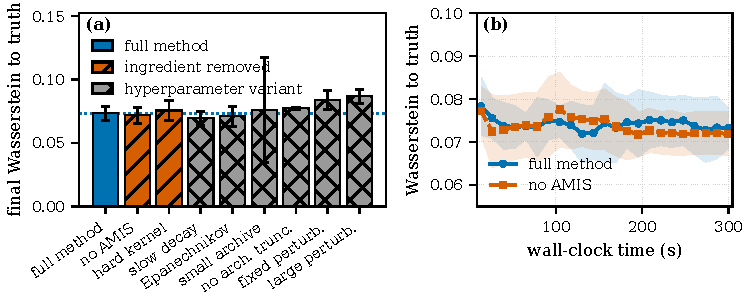
\includegraphics[width=\linewidth]{figures/fig_ablation.pdf}
\caption{Ablation on the Gaussian-mean benchmark (analytic posterior; $48$ workers, $300$\,s budget, $k=100$, five replicates, asynchronous method). (a) Final Wasserstein-to-truth for the full method (blue, solid), the two ingredient removals (vermillion, hatched: no AMIS, hard kernel), and hyperparameter variants (grey, cross-hatched); colour and hatch encode the class redundantly, error bars are $95\%$ CIs, and the dotted line marks the full-method mean. (b) AMIS isolation: full method vs.\ no-AMIS on a shared wall-clock grid (bands are $\pm1$ s.d.\ over replicates), zoomed to the converged regime; on this uniform-runtime analytic target the two variants track each other.}\label{fig:ablation}
\end{figure}

\subsection{Sensitivity}\label{sec:results-sensitivity}
Across the full hyperparameter grid \emph{on the Gaussian-mean benchmark} (the analytic-posterior sanity model) the asynchronous method's posterior quality is stable, with no region of catastrophic failure (Fig.~\ref{fig:sensitivity}). The Wasserstein distance to the true parameter stays within $\approx0.08$--$0.15$ across the grid (each cell averaged over five replicates and the two smooth kernels); the archive size $k$ matters only marginally \emph{for point quality at this dimension} (its effect on calibration in higher dimensions is a separate and much larger story, Table~\ref{tab:ks-sweep}), and quality degrades only mildly toward the largest perturbation scales and initial tolerances. The tolerance scheduler is inert under a smooth kernel --- the asynchronous selector chooses $\epsilon$ by ESS-retention bisection regardless of the scheduler type --- so we fixed it to the acceptance-rate rule rather than sweeping a variable that cannot change the smooth-kernel result. We therefore did not find delicate tuning necessary to reach the quality reported above \emph{on this benchmark}. We did not repeat the full grid on the costlier non-Gaussian benchmarks, so this robustness statement is scoped to the analytic-posterior model and to the qualitative trends observed there (scheduler-insensitive; mild, monotone sensitivity to perturbation scale and initial tolerance) rather than asserted as a general guarantee. Two further scope limits matter. This grid measures \emph{point quality} (Wasserstein to the truth) in \emph{one} dimension; it says nothing about calibration, and the archive size that looks inconsequential here is decisive for coverage in higher dimensions --- the dimension-resolved sweep of \S\ref{sec:results-validity} (Table~\ref{tab:ks-sweep}) finds a genuinely catastrophic region ($d=8$, $k=50$: coverage $0.29$ at the $0.50$ level) that a one-dimensional quality grid cannot see. ``No failure region'' should therefore be read as a statement about one-dimensional point quality only.

\begin{figure}[t]
\centering
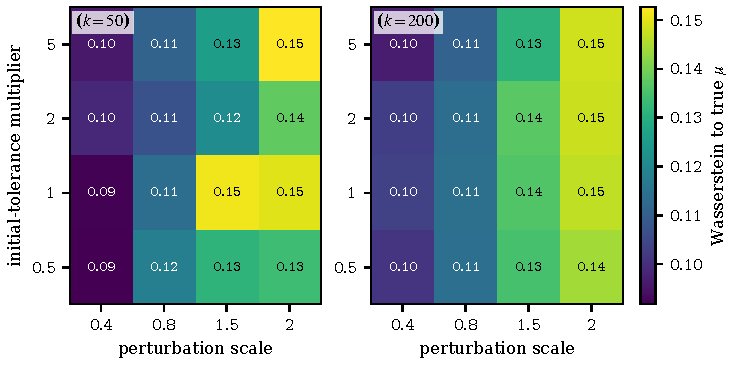
\includegraphics[width=\linewidth]{figures/fig_sensitivity_heatmap.pdf}
\caption{Hyperparameter sensitivity of the asynchronous method, measured by posterior quality (Wasserstein distance to the true $\mu$, lower is better; averaged over replicates and smoothing kernel). Each panel sweeps perturbation scale ($x$) against the initial-tolerance multiplier ($y$); panels are faceted by archive size $k$. Quality is stable across the grid (Wasserstein $\approx0.08$--$0.15$) with no failure region; the tolerance scheduler is inert under the smooth kernel and is held fixed, while larger perturbation scales degrade quality only mildly.}\label{fig:sensitivity}
\end{figure}

\section{Discussion}\label{sec:discussion}
The results support the three claims. Asynchronous execution helps most where it should: under a persistent straggler and under runtime heterogeneity, the generation barrier is the dominant cost and removing it preserves throughput that the synchronous baseline loses. For homogeneous, near-instantaneous simulators at large worker counts the asynchronous coordination overhead does not pay off: the multi-node Lotka--Volterra points, where the fair synchronous baseline overtakes the asynchronous method, make this honest boundary explicit. On the realistic Cellular Potts workload (the cost-bearing regime the design targets) the method scales almost linearly while the synchronous baseline, held at the generation barrier even when given a matching population, scales only sub-linearly --- at a small measured cost in posterior quality on that benchmark ($\S$\ref{sec:results-validity}), on a metric that penalizes the concentration the extra throughput buys.

\section{Limitations}\label{sec:limitations}
We are explicit about what \S\ref{sec:theory} does and does not give. (i) AMIS estimators are consistent but not finite-sample unbiased, since proposals depend on past particles; a local-decision rule in the spirit of \cite{paige2014cascade} that recovers finite-sample unbiasedness for ABC is future work. (ii) The bandwidth floor $\epsilon_\infty>0$ in Assumption~\ref{ass:stab} means the theorems characterize the smooth-ABC posterior at the limit bandwidth, not the exact posterior at $\epsilon=0$; and for the central limit theorem (though not for consistency) that limit must be \emph{deterministic}, since the centred integrand it is built on would otherwise vary with the run. Setting \texttt{min\_tol} bounds the limit below but only a schedule that reaches its floor makes it deterministic. The reported runs leave \texttt{min\_tol} unset and use the data-driven schedule, so neither holds, and the bandwidth a finite budget reaches is not an asymptotic limit at all. (iii) Theorems~\ref{thm:consistency}--\ref{thm:clt} are proved for $\mathcal{A}_\delta$, which draws a $\delta$ share of its candidates from the prior; the runs reported here do not, and Proposition~\ref{prop:tilt} gives the target the idealized version of what they run converges to instead --- equal to $\pi_{\epsilon_\infty}$ whenever bootstrap draws already carry a $\delta$ share of the history, and otherwise a tail-suppressed tilt of it, bounded by \eqref{eq:tilt-bound}. Three further deviations of the code from that idealization (a prior fallback recorded as an archive draw, underflow redraws, and an approximate truncation normalizer) are listed in \S\ref{sec:theory} and are not quantified. Making the two coincide is a one-line change to the candidate draw, but it changes the sampler and hence every measurement, so we report the gap rather than close it. The proposal-stabilization assumption itself (Assumption~\ref{ass:stab}) is assumed for the top-$k$ archive rule, not proved. (iv) Keeping every accepted particle (unlike pyABC's discard-latecomers rule) over-represents fast-simulator parameter regions in the raw archive. The parameter-coupled-runtime study (\S\ref{sec:results-hpc}, Fig.~\ref{fig:param-bias}) quantifies this: steepening the coupling cuts throughput as the fast region comes to dominate the raw counts, yet --- across the sweep, a steeper regime, and with or without AMIS --- neither the unweighted posterior mean nor the AMIS-reweighted posterior's mean drifts with the coupling (AMIS reshapes the tails, not the mean), and a drain-after-deadline test finds the completion-time censoring negligible in effect at these levels (numbers there). We therefore do not correct for it algorithmically and do not claim the AMIS reweighting cancels it: dividing by the proposal density corrects proposal adaptation, not selection by completion time, so a formal correction would need completion probabilities or an anytime-sampling argument, and a residual finite-sample effect at stronger couplings cannot be ruled out --- both left to future work. (v) The snapshot buffer is fixed at $S=20$; adaptive sizing is a natural extension. (vi) Simulation-based calibration of the reported posterior --- the full-history AMIS estimator \eqref{eq:posterior-estimator} --- shows it well calibrated in one dimension and robust to multimodality (retaining both modes of a bimodal target in ${\approx}86\%$ of trials), and conservative rather than over-confident on the four-dimensional g-and-k model, where it mildly \emph{over}-covers. This four-dimensional behaviour is a reporting-support effect, not a weighting or budget failure (\S\ref{sec:results-validity}): the efficient top-$k$ archive used for online proposal is over-concentrated and would under-cover, the full evaluated history is over-dispersed and over-covers, and coverage rises monotonically through nominal as the reported support grows from one to the other, so the calibrated posterior is bracketed between the two. We report the conservative full-history end by default; an intermediate reported support or a larger archive would tighten the four-dimensional report to nominal. The persistent defensive-mixture component of $\mathcal{A}_\delta$ (\S\ref{sec:theory}) would act in the same direction but for a different reason, and it is worth not conflating the two: the denominator's prior floor, which the runs already carry, suppresses the far tails of the reported posterior (Proposition~\ref{prop:tilt}) and so tightens it, whereas drawing from the defensive mixture as well removes that tilt and instead broadens the proposal's coverage. (vii) The synchronous baseline is matched on the ABC kernel and bandwidth schedule, but it still differs from our method in more than the barrier: it adds a probabilistic-rejection step, its generation length depends on the resulting acceptance probability, and it retains classical population weighting rather than the streaming estimator. Matching the kernel removes the acceptance \emph{rule} as a confound, and the \emph{barrierized twin} of \S\ref{sec:results-hpc} (Table~\ref{tab:twin}) closes the remaining gap on the straggler benchmark: the same propagator with a collective barrier before each breed runs $21$--$402\times$ slower than the asynchronous arm at unchanged posterior quality, so on that workload the gain is attributable to synchronization rather than merely dominated by it. The granularity objection --- that the twin synchronizes every $W$ evaluations, a finer generation than the baseline's population of $100$ --- is measured rather than assumed away: re-running the twin with the barrier coarsened to the baseline's population changes its throughput by less than $1\%$ at every slowdown from $5\times$ up, and matters ($2.3$--$3.3\times$) only at the controls where barrier latency and not straggler waiting is the bottleneck (Table~\ref{tab:twin}). The twin has since been repeated under runtime heterogeneity (Table~\ref{tab:twin-hetero}), where it costs $1.1\times$ at the $\sigma{=}0$ control and $25.3\times$ at $\sigma{=}2$ at the baseline-matched granularity, so the attribution now covers both synthetic HPC pathologies rather than only the sharpest one. That test also shows the cross-algorithm comparison to be conservative in the direction that matters: pyABC's own penalty grows only to $4.8\times$, because it discards latecomers instead of waiting for the slowest draw (item iv), so the barrier's unmitigated cost exceeds the gap we report against it. The twin has since also been run at scale on the Cellular Potts workload (Table~\ref{tab:twin-cpm}), and there the answer is more qualified. The barrier costs $1.9\times$ from one to four nodes and $2.8\times$ at eight, while pyABC's penalty over the same range grows from $2.4\times$ to $5.1\times$: the barrier is the largest single component we can identify, but it is not the whole gap, and the residual --- pyABC's probabilistic-rejection step, its classical population weighting, its own coordination --- grows with worker count. On the realistic simulator we therefore attribute the gain to synchronization only in part, and say so rather than generalizing the straggler result. The attribution now covers all three benchmarks on which we report systems gains, with the caveat that its strength differs across them: near-total under a straggler or heterogeneity, partial on Cellular Potts. Separately, the twin is a diagnostic rather than a robust implementation --- it intermittently deadlocks at $\ge192$ ranks (five hangs while collecting Table~\ref{tab:twin-cpm}), so replicates there needed retrying, though all twenty entries are complete runs. Separately, on a methodological note for reproducibility: the post-run retroactive estimator builds its denominator from $m\le S{+}1=21$ history-reconstructed proposals (with a defensive prior floor), not the full evaluated history; for a near-instantaneous simulator whose history reaches many millions of particles the pass is evaluated in bounded-memory chunks, which changes memory, not the estimate.

\section{Conclusion}\label{sec:conclusion}
We presented a generation-free, single-arrival-driven ABC algorithm that combines smooth-kernel ABC with streaming AMIS reweighting, is stateless and crash-recoverable, and integrates into Propulate's barrier-free island model. A precisely specified defensive-mixture form of its estimator is consistent and satisfies a central limit theorem with an explicit asymptotic variance and explicit rate conditions, proved directly rather than inherited; the posterior actually reported, a bounded-memory approximation evaluated over the full evaluated history, converges to a characterized and boundedly tilted version of the same target --- up to implementation deviations we enumerate rather than absorb --- and is validated empirically by simulation-based calibration --- well calibrated in low dimensions and under multimodality, and conservative rather than over-confident in higher dimensions, where we trace the residual miscalibration to how much of the evaluated history is reported (the efficient top-$k$ proposal would under-cover; the full history over-covers) rather than to the weighting. Against a synchronous pyABC baseline matched on the ABC kernel and bandwidth schedule, the method matches or exceeds the baseline's posterior quality on the analytic and Lotka--Volterra targets and trails it modestly on the weakly identified Cellular Potts target, while delivering substantial HPC benefits on heterogeneous and straggler-prone workloads, including that realistic Cellular Potts simulation. Asynchronous, generation-free ABC is a promising approach for large-scale simulator-based inference on modern HPC systems.

\bmhead{Acknowledgements}
\emph{To be added in the final version.}

\section*{Declarations}
\textbf{Funding} \\
\emph{To be added in the final version.}

\textbf{Conflict of interest/Competing interests} \\
The authors declare no competing interests.

\textbf{Ethics approval and consent to participate} \\
Not applicable.

\textbf{Consent for publication} \\
Not applicable.

\textbf{Data availability} \\
The experiment outputs backing every figure and table (raw per-particle records, per-rank phase-timing logs, and the throughput/utilization/coverage summary tables), together with the resolved run configurations, will be deposited in a public repository upon publication.

\textbf{Materials availability} \\
Not applicable.

\textbf{Code availability} \\
The full implementation (the stateless Propulate propagator, the matched-kernel pyABC baseline, and the analysis and plotting scripts that regenerate every figure and table from the deposited outputs) will be released in a public repository upon publication.

\textbf{Author contribution} \\
\emph{To be added in the final version.}

\begin{appendices}

\section{Proofs}\label{app:theory}

\subsection{Setting}\label{app:theory-setting}
Let $\mathcal{F}_{i-1}$ be the $\sigma$-field generated by everything realized before the $i$-th candidate is proposed, and write $\mathbb{E}_{i-1}[\cdot]=\mathbb{E}[\cdot\mid\mathcal{F}_{i-1}]$. Particles are indexed by \emph{proposal} time, not arrival time. This is what makes the martingale structure survive asynchronous execution: a worker forms its proposal from the history it has received at that moment, which is part of $\mathcal{F}_{i-1}$, so $q_i$ is $\mathcal{F}_{i-1}$-measurable and, under $\mathcal{A}_\delta$,
\begin{equation}
\theta_i\mid\mathcal{F}_{i-1}\sim q_i^\delta=\delta\pi+(1-\delta)q_i,
\qquad
\rho_i\mid\theta_i\sim p(\cdot\mid\theta_i).
\label{eq:app-conditional-law}
\end{equation}
Concurrency reorders the index set; it does not break \eqref{eq:app-conditional-law}. What it does affect is the reconstruction of the $q_{\tau_s}$ from a single rank's arrival-ordered log, which enters only through $\|\bar q_n-\bar q_\infty\|_\infty$ in Assumption~\ref{ass:stab}.

Write $\bar q^\star_n:=\tfrac1n\sum_{i\le n}q^\delta_i=\delta\pi+(1-\delta)\tfrac1n\sum_{i\le n}q_i$ for the empirical mixture the pooled sample was actually drawn from; the reported denominator $\bar q_n$ of \eqref{eq:snapshot-denominator} is an $m$-component stand-in for it. Let $\mathcal{Q}$ be the set of densities of the form \eqref{eq:snapshot-denominator} whose components satisfy Assumption~\ref{ass:class}. Elements of $\mathcal{Q}$ are parameterized by $p_q=(\text{means},\text{component weights},\text{covariances},\alpha)$ ranging over a compact set $P_q\subset\mathbb{R}^{D}$, $D=m\,(kd+k+d(d+1)/2)+m$.

\begin{lemma}[bounded weights]\label{lem:bounded}
Under Assumptions~\ref{ass:class}--\ref{ass:defensive}, $0\le W_{i,n}\le1/\delta$ for all $i\le n$ and all $n$, surely.
\end{lemma}
\begin{proof}
All components of \eqref{eq:snapshot-denominator} are non-negative, so $\bar q_n\ge\delta\pi$ pointwise on $\Theta$. Hence $W_{i,n}=\pi(\theta_i)K_{\epsilon_n}(\rho_i)/\bar q_n(\theta_i)\le K_{\epsilon_n}(\rho_i)/\delta\le1/\delta$, the last step by $K_\epsilon\le1$ (Assumption~\ref{ass:kernel}). The prior cancels exactly, so the bound needs neither a density-ratio condition nor a moment condition.
\end{proof}

\begin{lemma}[uniform SLLN for bounded martingale differences]\label{lem:uslln}
Let $P\subset\mathbb{R}^{D}$ be compact and $\{\psi_p\}_{p\in P}$ measurable functions on a measurable space $\mathcal{X}$ with $\sup_{p}\|\psi_p\|_\infty\le B$ and $|\psi_p(x)-\psi_{p'}(x)|\le\Lambda\|p-p'\|$ for every $x\in\mathcal{X}$. Let $(\xi_i)$ be $\mathcal{X}$-valued with $\xi_i$ $\mathcal{F}_i$-measurable. Then
\[
\sup_{p\in P}\Bigl|\tfrac1n\sum_{i\le n}\bigl(\psi_p(\xi_i)-\mathbb{E}_{i-1}\psi_p(\xi_i)\bigr)\Bigr|\;\longrightarrow\;0
\qquad\text{a.s.}
\]
\end{lemma}
\begin{proof}
Fix $p$. The variables $D^p_i:=\psi_p(\xi_i)-\mathbb{E}_{i-1}\psi_p(\xi_i)$ form a martingale difference sequence with $|D^p_i|\le2B$, so by the Azuma--Hoeffding inequality $\mathbb{P}(|\sum_{i\le n}D^p_i|\ge nt)\le2\exp(-nt^2/8B^2)$ for every $t>0$. Fix $\eta>0$ and let $P_\eta$ be a finite $\eta$-net of $P$, of cardinality at most $C_P\eta^{-D}$. A union bound gives $\mathbb{P}(\max_{p\in P_\eta}|\sum_{i\le n}D^p_i|\ge nt)\le2C_P\eta^{-D}\exp(-nt^2/8B^2)$, which is summable in $n$ (the net is fixed, so its cardinality does not grow with $n$); by Borel--Cantelli, $\limsup_n\max_{p\in P_\eta}|\tfrac1n\sum_{i\le n}D^p_i|\le t$ a.s. For arbitrary $p\in P$ pick $p'\in P_\eta$ with $\|p-p'\|\le\eta$; then $|D^p_i-D^{p'}_i|\le2\Lambda\eta$ by the Lipschitz hypothesis (which also bounds the conditional expectations), so $\limsup_n\sup_{p\in P}|\tfrac1n\sum_{i\le n}D^p_i|\le t+2\Lambda\eta$ a.s. Intersecting the almost-sure events over the countable family $t=1/r$, $\eta=1/j$ with $r,j\in\mathbb{N}$, gives the claim.
\end{proof}

\begin{lemma}[conditional-mean identity]\label{lem:condmean}
Let $\phi:\Theta\to\mathbb{R}$ be bounded measurable, let $r\in\{1,2\}$, and let $\epsilon\in[\epsilon_\infty,\epsilon_0]$ and the density $q\ge\delta\pi$ be either deterministic or $\mathcal{F}_{i-1}$-measurable. Then under \eqref{eq:app-conditional-law}, writing $L^{(1)}_\epsilon:=L_\epsilon$,
\[
\mathbb{E}_{i-1}\!\left[\frac{\phi(\theta_i)\,K_\epsilon(\rho_i)^{r}}{q(\theta_i)^{r}}\right]
=\int_\Theta \phi\,L^{(r)}_\epsilon\,\frac{q^\delta_i}{q^{r}}\,d\theta .
\]
\end{lemma}
\begin{proof}
Condition on $\mathcal{F}_{i-1}$, given which $\epsilon$ and $q$ are constants, and integrate first over $\rho_i\sim p(\cdot\mid\theta_i)$, which gives the factor $L^{(r)}_\epsilon(\theta_i)=\mathbb{E}[K_\epsilon(\rho)^r\mid\theta_i]$, then over $\theta_i\sim q^\delta_i$. The $\mathcal{F}_{i-1}$-measurable case is what Steps~2 and 3 of the proof of Theorem~\ref{thm:clt} need; an $\mathcal{F}_\infty$-measurable $q$ --- such as the limit $\bar q_\infty$ --- would \emph{not} be admissible here, which is why that proof centres on predictable proxies rather than on the limit. Fubini applies because the integrand is bounded by $\|\phi\|_\infty/(\delta\pi_-)^{r}$. The case $r=1$, $\phi=\pi h$ is the one used for first moments; $r=2$, $\phi=\pi^2h^2$ gives the conditional second moments of Step~3(b) and Corollary~\ref{cor:ci}.
\end{proof}

\paragraph{The class used below.} Take $\mathcal{X}=\Theta\times[0,\infty)$, $\xi_i=(\theta_i,\rho_i)$, and, for a fixed bounded measurable $h$,
\begin{equation}
\psi_{(\epsilon,p_q)}(\theta,\rho):=\frac{\pi(\theta)\,h(\theta)\,K_\epsilon(\rho)}{q_{p_q}(\theta)},
\qquad
(\epsilon,p_q)\in P:=[\epsilon_\infty,\epsilon_0]\times P_q .
\label{eq:app-class}
\end{equation}
$P$ is compact and $\sup_P\|\psi\|_\infty\le\|h\|_\infty/\delta$ by the computation of Lemma~\ref{lem:bounded}. For the Lipschitz hypothesis: each truncated component density $\varphi(\theta;\mu_j,\Sigma)/Z(\mu_j,\Sigma)$ has parameter-derivatives bounded uniformly over $\theta\in\Theta$, because $\Theta$ is compact, $\sigma_-^2I\preceq\Sigma\preceq\sigma_+^2I$ bounds $\varphi$ and its derivatives, and the truncation mass is bounded below, $Z(\mu_j,\Sigma)\ge c_0>0$, uniformly for $\mu_j\in\Theta$: this is where Assumption~\ref{ass:class}'s box hypothesis is used --- for a radius $r$ no larger than half the narrowest side of $\Theta$, one inward orthant of $B(\mu_j,r)$, a $2^{-d}$ fraction of its volume, lies in $\Theta$ for every $\mu_j\in\Theta$, and $\Sigma\preceq\sigma_+^2I$ bounds the Gaussian density below on that ball; compactness of $\Theta$ alone would not give this. Hence every $q\in\mathcal{Q}$ obeys $\delta\pi_-\le q\le q_+<\infty$ and $q\mapsto q(\theta)$ is Lipschitz in $p_q$ uniformly in $\theta$; so is $1/q$, since $q$ is bounded away from $0$. With $K_\epsilon$ Lipschitz in $\epsilon$ (Assumption~\ref{ass:kernel}) and $\pi h$ bounded, \eqref{eq:app-class} satisfies the hypotheses of Lemma~\ref{lem:uslln}. Note that $(\epsilon_n,\bar q_n)\in P$ for every $n$, and that $\bar q_\infty\ge\delta\pi$ by taking uniform limits.

\subsection{Proof of Theorem~\ref{thm:consistency}}\label{app:theory-consistency}
Fix a bounded measurable $h$, let $\widehat p_n:=(\epsilon_n,\bar q_n)\in P$, and define, for each \emph{fixed} $p\in P$, $\Gamma_i(p):=\mathbb{E}_{i-1}[\psi_p(\xi_i)]$ and $\bar\Gamma_n(p):=\tfrac1n\sum_{i\le n}\Gamma_i(p)$. On the almost-sure event of Lemma~\ref{lem:uslln} the bound holds simultaneously for all $p\in P$, so the \emph{function} $\bar\Gamma_n$ may be evaluated at the random $\widehat p_n$:
\begin{equation}
\frac1n\sum_{i\le n}W_{i,n}h(\theta_i)
=\bar\Gamma_n(\widehat p_n)+o(1)
\overset{\text{Lem.\ \ref{lem:condmean}}}{=}\int_\Theta \pi\,h\,L_{\epsilon_n}\,\frac{\bar q^\star_n}{\bar q_n}\,d\theta+o(1)
\quad\text{a.s.},
\label{eq:app-consistency-main}
\end{equation}
using $\tfrac1n\sum_{i\le n}q^\delta_i=\bar q^\star_n$. The middle term is the function $\bar\Gamma_n(\cdot)$ evaluated at $\widehat p_n$ and must not be read as $\mathbb{E}_{i-1}[\psi_{\widehat p_n}(\xi_i)]$: $\widehat p_n$ depends on draws after $i$, is not $\mathcal{F}_{i-1}$-measurable, and that conditional expectation is not what Lemma~\ref{lem:uslln} controls. Split the integral against $\int\pi hL_{\epsilon_\infty}$:
\[
\Bigl|\int \pi h L_{\epsilon_n}\tfrac{\bar q^\star_n}{\bar q_n}-\int\pi hL_{\epsilon_\infty}\Bigr|
\le \|h\|_\infty\,\pi_+|\Theta|\,\Bigl[\,R\,L_K|\epsilon_n-\epsilon_\infty|
+\Bigl\|\tfrac{\bar q^\star_n}{\bar q_n}-1\Bigr\|_\infty\Bigr],
\]
where $R:=(\delta\pi_++(1-\delta)q_+)/(\delta\pi_-)$ bounds $\bar q^\star_n/\bar q_n$, using $|L_{\epsilon_n}-L_{\epsilon_\infty}|\le L_K|\epsilon_n-\epsilon_\infty|$ (Assumption~\ref{ass:kernel} and Jensen) and $L_{\epsilon_\infty}\le1$. The first term vanishes because $\epsilon_n\to\epsilon_\infty$; the second is exactly \eqref{eq:stab-consistency}. (If one prefers to assume proposal convergence outright, it implies \eqref{eq:stab-consistency}: $\|q_n-q_\infty\|_\infty\to0$ gives $\|\bar q^\star_n-\bar q_\infty\|_\infty\to0$ by Ces\`aro averaging, and $\bar q_n\ge\delta\pi_-$ converts the resulting sup-norm difference into the sup-norm ratio bound.) Hence $\tfrac1n\sum_iW_{i,n}h(\theta_i)\to\int\pi hL_{\epsilon_\infty}$ a.s. Applying this with $h=f$ and with $h\equiv1$ and dividing --- legitimate since $Z_{\epsilon_\infty}=\int\pi L_{\epsilon_\infty}>0$ --- gives $\widehat\pi_n(f)\to\pi_{\epsilon_\infty}(f)$ a.s.\hfill$\square$

\begin{remark}\label{rem:weaker-c4}
The proof used Assumption~\ref{ass:stab} only through $\|\bar q^\star_n/\bar q_n-1\|_\infty\to0$ and $\epsilon_n\to\epsilon_\infty$. Consistency therefore holds under that weaker primitive condition --- the reported denominator must track the mixture the sample was actually drawn from --- whether or not the proposal sequence itself converges. This is the content Condition~(C4) of earlier drafts was missing: convergence to the \emph{idealized} cumulative mixture is not what the argument needs, and on its own does not deliver it.
\end{remark}

\subsection{Proof of Theorem~\ref{thm:clt} and Corollary~\ref{cor:ci}}\label{app:theory-clt}
Let $g:=f-\pi_{\epsilon_\infty}(f)$, which is bounded with $\int\pi gL_{\epsilon_\infty}=0$. Since $\sum_iW_{i,n}g(\theta_i)=(\sum_iW_{i,n})(\widehat\pi_n(f)-\pi_{\epsilon_\infty}(f))$ identically and $\tfrac1n\sum_iW_{i,n}\to Z_{\epsilon_\infty}>0$ a.s.\ (Theorem~\ref{thm:consistency} with $h\equiv1$), by Slutsky's theorem --- which preserves stable convergence --- it suffices to prove
\begin{equation}
S_n:=\frac{1}{\sqrt n}\sum_{i\le n}\frac{\pi(\theta_i)g(\theta_i)K_{\epsilon_n}(\rho_i)}{\bar q_n(\theta_i)}
\;\longrightarrow\;\mathcal{N}(0,v^2)\ \text{stably},
\qquad
v^2:=\int_\Theta\frac{\pi^2g^2L^{(2)}_{\epsilon_\infty}}{\bar q_\infty}\,d\theta,
\label{eq:app-clt-target}
\end{equation}
after which $\sigma^2_f=v^2/Z^2_{\epsilon_\infty}$, which is \eqref{eq:clt-variance}.

\emph{Step 1 (replacing the parameters by predictable proxies).} $\bar q_\infty$ and $\epsilon_\infty$ are in general only $\mathcal{F}_\infty$-measurable, so an array built from them is \emph{not} adapted and Lemma~\ref{lem:condmean} does not apply to it. We therefore centre on the predictable pair instead: let $\bar q_{i-1}\in\mathcal{Q}$ be the denominator \eqref{eq:snapshot-denominator} formed from the first $i-1$ draws and $\epsilon_{i-1}$ the bandwidth in force at the $i$-th proposal, both $\mathcal{F}_{i-1}$-measurable, and put
\[
V_i:=\frac{\pi(\theta_i)\,g(\theta_i)\,K_{\epsilon_{i-1}}(\rho_i)}{\bar q_{i-1}(\theta_i)} .
\]
Since $\bar q_n,\bar q_{i-1}\ge\delta\pi_-$ and $K\le1$, and $|\epsilon_n-\epsilon_{i-1}|\le|\epsilon_n-\epsilon_\infty|+|\epsilon_{i-1}-\epsilon_\infty|$ (likewise for $\bar q$),
\[
\Bigl|S_n-\tfrac{1}{\sqrt n}\sum_{i\le n}V_i\Bigr|
\le C\sqrt n\bigl(|\epsilon_n-\epsilon_\infty|+\|\bar q_n-\bar q_\infty\|_\infty\bigr)
+\frac{C}{\sqrt n}\sum_{i\le n}\bigl(|\epsilon_{i-1}-\epsilon_\infty|+\|\bar q_{i-1}-\bar q_\infty\|_\infty\bigr)
\]
with $C=\|g\|_\infty\pi_+\max\{L_K/(\delta\pi_-),(\delta\pi_-)^{-2}\}$, and both brackets vanish by \eqref{eq:rate}. This step is what the rates buy; the remainder of the proof never touches $\bar q_n$ or $\epsilon_n$ again.

\emph{Step 2 (drift).} Lemma~\ref{lem:condmean} with $r=1$, $\phi=\pi g$ applies to $V_i$ because $(\epsilon_{i-1},\bar q_{i-1})$ is $\mathcal{F}_{i-1}$-measurable and $g$ is a fixed function, $\epsilon_\infty$ being deterministic under the central-limit clause of Assumption~\ref{ass:stab}; with $\int\pi gL_{\epsilon_\infty}=0$,
\[
c_i:=\mathbb{E}_{i-1}V_i=\int\pi g\Bigl(L_{\epsilon_{i-1}}\frac{q^\delta_i}{\bar q_{i-1}}-L_{\epsilon_\infty}\Bigr)d\theta,
\]
\[
|c_i|\le C'\bigl(|\epsilon_{i-1}-\epsilon_\infty|+\|q_i-q_\infty\|_\infty+\|\bar q_{i-1}-\bar q_\infty\|_\infty\bigr),
\]
$C'$ depending only on $\|g\|_\infty,\pi_\pm,\delta,|\Theta|,L_K$. The second half of \eqref{eq:rate} is exactly the statement that $n^{-1/2}\sum_{i\le n}$ of that bound tends to zero, so $n^{-1/2}\sum_{i\le n}c_i\to0$. (Under the sufficient condition that each of the three terms is $O(i^{-1/2-a})$ this holds in each of the cases $a<1/2$, $a=1/2$, $a>1/2$, where the partial sums are $O(n^{1/2-a})$, $O(\log n)$ and $O(1)$ respectively.)

\emph{Step 3 (martingale CLT).} Let $X_{n,i}:=n^{-1/2}(V_i-c_i)$, a martingale difference array with respect to the filtration $(\mathcal{F}_i)$, which does not depend on $n$ and is therefore nested. Two conditions:
\emph{(a) Conditional Lindeberg.} $|X_{n,i}|\le2\|g\|_\infty\pi_+/(\delta\pi_-\sqrt n)$ surely, so for every $\eta>0$ the truncated sum $\sum_i\mathbb{E}_{i-1}[X^2_{n,i}\mathbf{1}\{|X_{n,i}|>\eta\}]$ is exactly zero for all $n$ large. The defensive floor makes this step trivial where an unbounded-weight scheme would need a uniform-integrability argument.
\emph{(b) Conditional variance.} Lemma~\ref{lem:condmean} with $r=2$, $\phi=\pi^2g^2$ gives
\[
\mathbb{E}_{i-1}V_i^2=\int\frac{\pi^2g^2L^{(2)}_{\epsilon_{i-1}}}{\bar q^2_{i-1}}\,q^\delta_i\,d\theta
=v^2+R_i,
\]
\[
v^2=\int\frac{\pi^2g^2L^{(2)}_{\epsilon_\infty}}{\bar q_\infty}\,d\theta,
\qquad
|R_i|\le C''\bigl(|\epsilon_{i-1}-\epsilon_\infty|+\|q_i-q_\infty\|_\infty+\|\bar q_{i-1}-\bar q_\infty\|_\infty\bigr).
\]
The bound on $|R_i|$ has vanishing Ces\`aro average, a fortiori from \eqref{eq:rate}, so $\tfrac1n\sum_{i\le n}\mathbb{E}_{i-1}V^2_i\to v^2$ a.s.; with $\tfrac1n\sum_ic^2_i\to0$ from Step 2,
$\sum_i\mathbb{E}_{i-1}X^2_{n,i}=\tfrac1n\sum_i(\mathbb{E}_{i-1}V^2_i-c^2_i)\to v^2$ a.s. Note that $v^2$ is permitted to be random here --- an $\mathcal{F}_\infty$-measurable limit of the conditional variances is exactly the setting the martingale CLT below covers, and it is only inside $\mathbb{E}_{i-1}$ that predictability was needed.
The martingale central limit theorem for arrays with nested $\sigma$-fields, in its conditional-variance form \cite[Cor.~3.1, pp.~58--59]{hall1980martingale}, then gives $\sum_iX_{n,i}\to\mathcal{N}(0,v^2)$ stably; the convergence is stable rather than merely distributional precisely because $v^2$ is $\mathcal{F}_\infty$-measurable and possibly random. Combining Steps 1--3 gives \eqref{eq:app-clt-target}.\hfill$\square$

\begin{proof}[Proof of Corollary~\ref{cor:ci}]
Write $\widehat\sigma^2_n=[\tfrac1n\sum_iW^2_{i,n}(f(\theta_i)-\widehat\pi_n(f))^2]\,/\,[\tfrac1n\sum_iW_{i,n}]^2$. In the numerator, $(f-\widehat\pi_n(f))^2=g^2+2g(\pi_{\epsilon_\infty}(f)-\widehat\pi_n(f))+(\pi_{\epsilon_\infty}(f)-\widehat\pi_n(f))^2$, and $W_{i,n}\le1/\delta$ with $\widehat\pi_n(f)\to\pi_{\epsilon_\infty}(f)$ a.s.\ (Theorem~\ref{thm:consistency}), so the cross terms vanish and it suffices to treat $\tfrac1n\sum_iW^2_{i,n}g(\theta_i)^2$. Apply Lemma~\ref{lem:uslln} to the class $\psi_{(\epsilon,p_q)}(\theta,\rho)=\pi(\theta)^2g(\theta)^2K_\epsilon(\rho)^2/q_{p_q}(\theta)^2$, which is bounded by $\|g\|^2_\infty/\delta^2$ and Lipschitz in $(\epsilon,p_q)$ by the same argument as \eqref{eq:app-class}; the substitution of $\widehat p_n$ used in \eqref{eq:app-consistency-main}, followed by Lemma~\ref{lem:condmean} with $r=2$, $\phi=\pi^2g^2$ (a fixed function, since $\epsilon_\infty$ is deterministic), gives
$\tfrac1n\sum_iW^2_{i,n}g^2(\theta_i)=\int\pi^2g^2L^{(2)}_{\epsilon_n}\,\bigl(\bar q^\star_n/\bar q_n\bigr)\,\bar q_n^{-1}+o(1)$,
and $\epsilon_n\to\epsilon_\infty$, $\|\bar q^\star_n/\bar q_n-1\|_\infty\to0$ and $\|\bar q_n-\bar q_\infty\|_\infty\to0$ (the last from \eqref{eq:rate}) send this to $v^2$ a.s. The denominator tends to $Z^2_{\epsilon_\infty}$, so $\widehat\sigma^2_n\to v^2/Z^2_{\epsilon_\infty}=\sigma^2_f$ a.s. Because the convergence in Theorem~\ref{thm:clt} is stable, the pair $(\sqrt n(\widehat\pi_n(f)-\pi_{\epsilon_\infty}(f)),\widehat\sigma_n)$ converges jointly to $(\sigma_f\mathcal{Z},\sigma_f)$ --- stable convergence is exactly joint convergence with every $\mathcal{F}_\infty$-measurable variable, and $\sigma_f$ is one --- so with $\sigma_f>0$ a.s.\ the continuous mapping theorem gives $\mathcal{Z}\sim\mathcal{N}(0,1)$ as the limit of the ratio. Marginal convergence to a mixed normal alone would not suffice.
\end{proof}

\begin{remark}[growing snapshot count]\label{rem:growing-m}
Nothing above requires $m$ to be fixed except the compactness and fixed dimension $D$ of $P_q$. If $m=m_n\to\infty$, run the proof of Lemma~\ref{lem:uslln} with an $n$-dependent net: the union bound costs $D_n\log(1/\eta_n)$ with $D_n=\Theta(m_n)$, and the Lipschitz constant over the mixture weights grows at most polynomially in $m_n$, so choosing $\eta_n\to0$ fast enough leaves the Borel--Cantelli step summable for any $m_n=o(n/\log n)$. In that regime the snapshot clause of Assumption~\ref{ass:stab} follows from $V_n/m_n\to0$, with $V_n=\sum_{i<n}\|q_{i+1}-q_i\|_\infty$ the total variation of the proposal path, rather than having to be assumed: the draw-proportional $m_n$-point mixture is then a converging quadrature of the empirical mixture. The retroactive pass costs $\mathcal{O}(n\,m_n\,k)$.
\end{remark}

\subsection{Proof of Proposition~\ref{prop:tilt}}\label{app:theory-tilt}
Under $\mathcal{A}_0$ the conditional law \eqref{eq:app-conditional-law} reads $\theta_i\mid\mathcal{F}_{i-1}\sim q_i$ outside the bootstrap phase and $\sim\pi$ inside it, so the empirical draw mixture is $\bar q^\star_n=\nu_n\pi+(1-\nu_n)\tfrac{1}{n-n\nu_n}\sum_{i\in\mathrm{arch}}q_i\to\nu_\infty\pi+(1-\nu_\infty)q_\infty$ uniformly, while $\bar q^{\mathrm{fl}}_n\to\bar q^{\mathrm{fl}}_\infty=w\pi+(1-w)q_\infty$ with $w=\max(\nu_\infty,\delta)$. Lemma~\ref{lem:bounded} still applies, because $\bar q^{\mathrm{fl}}_n\ge\delta\pi$; so do Lemmas~\ref{lem:uslln} and \ref{lem:condmean}. Repeating \eqref{eq:app-consistency-main} verbatim gives
$\tfrac1n\sum_iW_{i,n}h(\theta_i)\to\int\pi hL_{\epsilon_\infty}r_\infty$ with $r_\infty=\bar q^\star_\infty/\bar q^{\mathrm{fl}}_\infty$, and dividing the $h=f$ and $h\equiv1$ limits gives \eqref{eq:tilt}. If $\nu_\infty\ge\delta$ then $w=\nu_\infty$, the two mixtures coincide and $r_\infty\equiv1$.

For \eqref{eq:tilt-bound}, suppose $\nu_\infty<\delta$ and write $u:=q_\infty/\pi$. Then
\[
r_\infty-1=\frac{\nu_\infty+(1-\nu_\infty)u}{\delta+(1-\delta)u}-1=\frac{(\delta-\nu_\infty)(u-1)}{\delta+(1-\delta)u},
\]
so on $\{u\ge c\}$, splitting at $u=1$ and bounding each branch, $|r_\infty-1|\le(\delta-\nu_\infty)\max\{(1-\delta)^{-1},(\delta+(1-\delta)c)^{-1}\}=:\eta_A$. Globally $r_\infty$ lies between $\nu_\infty/\delta$ and $(1-\nu_\infty)/(1-\delta)$, so $|r_\infty-1|\le1$ for $\delta\le1/2$, whence $\zeta_0:=\pi_{\epsilon_\infty}(|r_\infty-1|)\le\eta_A+\pi_{\epsilon_\infty}(A^c)=:\zeta$. Finally, for bounded $f$,
\[
\widetilde\pi_{\epsilon_\infty}(f)-\pi_{\epsilon_\infty}(f)
=\frac{\pi_{\epsilon_\infty}\!\left(f(r_\infty-1)\right)-\pi_{\epsilon_\infty}(f)\,\pi_{\epsilon_\infty}(r_\infty-1)}{\pi_{\epsilon_\infty}(r_\infty)},
\]
whose modulus is at most $2\|f\|_\infty\zeta_0/(1-\zeta_0)$ since $\pi_{\epsilon_\infty}(r_\infty)\ge1-\zeta_0$; taking the supremum over $\|f\|_\infty\le1$ and halving bounds the total variation by $\zeta_0/(1-\zeta_0)$. As $x\mapsto x/(1-x)$ increases on $[0,1)$, this is at most $\zeta/(1-\zeta)$ \emph{provided} $\zeta<1$, which is the form stated in \eqref{eq:tilt-bound}; when $\zeta\ge1$ the bound degenerates and only the trivial $\|\cdot\|_{\mathrm{TV}}\le1$ survives.\hfill$\square$

\subsection{Status of each assumption in the implementation}\label{app:theory-status}
\begin{table}[h]
\caption{What the implementation guarantees, what it assumes, and what it violates. ``By construction'' means the code enforces the property for every run, not that it was checked post hoc.}\label{tab:assumption-status}
\centering
\begin{tabular}{@{}p{0.20\textwidth}p{0.13\textwidth}p{0.57\textwidth}@{}}
\toprule
Assumption & Status & Basis \\
\midrule
\ref{ass:kernel} kernel & by construction & Gaussian ($L_K=2/e\epsilon_\infty$) and Epanechnikov ($2/\epsilon_\infty$) are peak-normalized and Lipschitz in $\epsilon$ on $[\epsilon_\infty,\epsilon_0]$. The hard indicator is not, and is excluded from the theory. \\
\ref{ass:class} proposal class & by construction, \emph{except} the normalizer & The prior support is a box and the archive lies in it, so component means do; the covariance carries an additive jitter $10^{-9}\mathrm{tr}(\widehat\Sigma)/d+10^{-12}\bar b^2$ ($\bar b^2$ the mean squared box width), whose second term is a run-independent floor, giving $\sigma_-^2>0$, and $\sigma_+^2$ follows from the archive lying in a bounded box. The truncation \emph{normalizer}, however, is the product of per-axis in-box masses --- exact for a diagonal covariance, increasingly accurate as a component's mass moves away from the faces relative to its own scale, an approximation in general --- so the evaluated component density is not exactly the one sampled from. \\
\ref{ass:defensive} floor, denominator & by construction & The retroactive denominator floors the prior component's mass at $\delta=0.5/(m{+}1)$ (Appendix~\ref{app:implementation}), so $\bar q_n\ge\delta\pi$ and Lemma~\ref{lem:bounded} applies to every reported posterior. \\
\ref{ass:defensive} floor, sampler & \textbf{not satisfied} & The reported runs draw from the prior only in the bootstrap phase, so $\nu_n\downarrow0<\delta$; \eqref{eq:defensive-proposal} is the one-line change that removes this. Proposition~\ref{prop:tilt} isolates the consequence for the idealized $\mathcal{A}_0$; the code additionally caps the in-box rejection at $992$ attempts (tilting the component weights and emitting the residual as a bandwidth-stamped prior draw) and redraws underflowing candidates, emitting the last one regardless. Neither is shown to vanish asymptotically; see \S\ref{sec:theory}. \\
\ref{ass:stab} stabilization & assumed & Not implied by the top-$k$ rule: the archive keeps improving as better particles arrive, and we do not prove it settles. Two further approximations enter here rather than separately --- the asynchronous replay of the proposal sequence, and the $m$-snapshot quadrature of the proposal path (Remark~\ref{rem:growing-m}). \\
\ref{ass:stab} $\epsilon_\infty>0$ (deterministic, for the CLT only) & \textbf{not satisfied} & A strictly positive \texttt{min\_tol} forces $\epsilon_\infty\ge\texttt{min\_tol}>0$, since $\{\epsilon_n\}$ is non-increasing and clipped from below, which is all Theorem~\ref{thm:consistency} needs. Theorem~\ref{thm:clt} additionally needs $\epsilon_\infty$ deterministic, so that $f-\pi_{\epsilon_\infty}(f)$ is a fixed function; a floor alone does not give that, since a monotone data-driven schedule may settle above it at a run-dependent value. A schedule that reaches its floor in finite time does, and makes the $\epsilon$ terms of \eqref{eq:rate} vanish identically. The runs reported here leave \texttt{min\_tol} unset (zero is accepted), so neither part holds and the bandwidth a finite budget reaches is not an asymptotic $\epsilon_\infty$ at all. \\
\ref{ass:stab} rate \eqref{eq:rate} & assumed & Needed only in Step 1 and Step 2 of the proof of Theorem~\ref{thm:clt}; consistency does not use it. \\
\botrule
\end{tabular}
\end{table}

\section{Implementation Details}\label{app:implementation}

\paragraph{Tolerance schedulers.} Every scheduler is a pure function of the evaluated history and is \emph{monotone by construction}: the propagator clips any proposed bandwidth above the history-reconstructed running minimum $\epsilon_{\text{hist}}$ (\S\ref{sec:method-tolerance}), so the effective tolerance can only decrease. Let $m$ denote the extra-individual margin (default $m=k$). The three base rules act on the individuals \emph{within} the current bandwidth, i.e.\ the hard-threshold set $\{i:\rho_i<\epsilon\}$. (This bandwidth-membership count is used \emph{only} to drive the tolerance schedule; it is distinct from the smooth-kernel weight $K_\epsilon(\rho_i)$ that defines the proposal mixture and the reported posterior, for which every evaluated particle contributes continuously. We avoid the word ``accepted'' here precisely because acceptance is probabilistic under a smooth kernel.):
\begin{itemize}
\item \textbf{Quantile.} $\epsilon \leftarrow$ the lower-rank (non-interpolated) $p$-th percentile of the accepted losses, default $p=50$; applied only once at least $k+m$ individuals are accepted.
\item \textbf{Geometric decay.} $\epsilon \leftarrow \epsilon_0\,\gamma^{\,e}$ after each completed epoch $e$ of $k+m$ accepted individuals, default $\gamma=0.9$.
\item \textbf{Acceptance rate.} Over a sliding window of the most recent $k+m$ individuals, if the acceptance rate exceeds $r_{\text{hi}}$ (default $0.3$) tighten by a factor $0.9$, otherwise hold; the rule never expands $\epsilon$ (the low-rate guard $r_{\text{lo}}=0.1$ simply holds).
\end{itemize}
With a smooth (Gaussian or Epanechnikov) kernel the schedulers run in a \emph{kernel-aware} mode: instead of the hard $\rho<\epsilon$ count, $\epsilon$ is chosen by bisection so that the per-step kernel-weighted effective-sample-size retention ratio meets a target (default $0.95$), which keeps the bandwidth schedule comparable across kernel choices.

\paragraph{Proposal covariance.} The archive $A_n$ is the top-$k$ history members by smallest discrepancy. Component weights are formed in log-space as $\tilde W_j \propto w_j\,K_{\epsilon_n}(\rho_j)$ and normalised (a uniform fallback is used if all smooth weights underflow). The perturbation covariance is $\Sigma_n = s\,[\,\widehat{\mathrm{Cov}}_{\tilde W}(A_n) + \lambda_n I\,]$ with $s$ the \texttt{perturbation\_scale} and a two-part jitter $\lambda_n = 10^{-9}\,\mathrm{tr}\,\widehat{\mathrm{Cov}}_{\tilde W}(A_n)/d + 10^{-12}\,\bar b^2$, where $\bar b^2$ is the mean squared prior-box width; it is Cholesky-factored once per call. The first term is scale-aware, so a tightly converged archive (marginal standard deviation ${\sim}10^{-4}$) is not swamped by the floor as a fixed $10^{-6}$ would swamp it; the second is a run-independent absolute floor that keeps the matrix factorable for a degenerate archive and supplies the uniform lower spectral bound Assumption~\ref{ass:class} needs (Table~\ref{tab:assumption-status}). Each mixture component is truncated to the prior box, with its log normalising mass computed analytically so the proposal integrates to one on the support.

\paragraph{Matched pyABC acceptor.} For the synchronous baseline, pyABC's \texttt{UniformAcceptor} is replaced, for smooth kernels, by a probabilistic-rejection acceptor that accepts a candidate of discrepancy $\rho$ with probability $K_{\epsilon}(\rho)$ (peak-normalised so $K_{\epsilon}(0)=1$), using the \emph{same} kernel $K_{\epsilon}$ as the asynchronous side; the hard kernel falls back to \texttt{UniformAcceptor}. The rejection step of each replicate draws from an independently seeded generator. This is the sense in which the kernel and acceptor are matched across methods (\S\ref{sec:implementation}).

\paragraph{Bounded-memory posterior estimator.} The retroactive AMIS estimator \eqref{eq:posterior-estimator} evaluates the snapshot denominator $\bar q_n$ --- a draw-proportional mixture of $m\le S{+}1=21$ history-reconstructed proposals with a defensive prior component (mass floored at $0.5/(m{+}1)$) --- at each of the $n$ evaluated particles, at total cost $\mathcal{O}(n\,m\,k)=\mathcal{O}(nk)$ with $m$ fixed. The snapshots are taken draw-proportionally from the reconstructed archive (indices $0,\text{step},2\,\text{step},\dots$ with $\text{step}=\max(1,\lfloor|\text{archive}|/S\rfloor)$), plus the most recent archive-phase proposal if it is not already among them --- hence $m\le S{+}1=21$ rather than $S$. For near-instantaneous simulators the history reaches $\mathcal{O}(10^7)$ particles, so the pass is accumulated in chunks of $2^{16}=65{,}536$ history points: peak memory is $\mathcal{O}(\text{chunk}\cdot m\cdot k)$ rather than $\mathcal{O}(n)$. Each particle's denominator is evaluated independently within a single chunk (there is no log-sum-exp reduction \emph{across} chunk boundaries), so chunking changes memory, not the value, and the result is bit-identical to the unchunked computation. Measured on the largest history (Gaussian-mean, $n\approx3\times10^7$ evaluated particles, $k=100$, $m=20$), the one-time retroactive pass runs in ${\approx}20$~minutes on a single core with ${\approx}0.3$\,GB peak memory (independent of $n$; the intermediate is one $2^{16}$-point chunk) and parallelizes trivially across evaluation points; it runs after the timed budget and is excluded from the throughput measurements by design. For a near-instantaneous simulator this is comparable to the timed budget itself --- non-trivial though bounded --- whereas for cost-bearing simulators, whose histories are orders of magnitude shorter, it is negligible against the simulation time.

\section{Additional Experimental Protocol}\label{app:protocol}

\paragraph{Seeding.} Each experiment derives its replicate seeds deterministically from a single base seed via \texttt{make\_seeds}: a \texttt{random.Random(base)} stream emits unique non-negative 31-bit integers, one per replicate, portable across platforms and independent of any global RNG state. Derived seeds (observed-data generation, the pyABC rejection step) use a structured BLAKE2b hash (\texttt{stable\_seed}) of their inputs, so identical inputs reproduce identical seeds across fresh and resumed (\texttt{--extend}) runs.

\paragraph{Crash recovery (kill-and-resume).} We test the crash-recoverability claim of \S\ref{sec:method-constraints} directly. On the Gaussian-mean benchmark ($4$ workers, a $1.2\times10^{5}$-simulation budget) we compare a clean uninterrupted run against a run that is hard-killed (\texttt{SIGKILL} of the entire worker process group) partway through inference and then relaunched with an identical command; recovery reloads the periodic population checkpoint and resumes from the next generation. The resumed run recovers the analytic posterior mean --- absolute error $7.6\times10^{-3}$, against $7.5\times10^{-4}$ for the clean run --- and completes the same total simulation budget with no duplicated records. It is \emph{not} a bit-identical replay: the two reported posterior means differ by $6.9\times10^{-3}$, because the candidate generator is re-seeded from its (replicate, rank) key on restart rather than checkpointed, and MPI arrival order is not deterministic. This is exactly the sense in which the method is ``reproducible up to MPI arrival order'' (\S\ref{sec:method-constraints}): recovery yields a \emph{valid} posterior trajectory over the actual evaluated history, not the identical one. In this instance the kill landed \emph{during} a checkpoint write and truncated the primary checkpoint; recovery fell back to the previous-state backup that the dumper writes before overwriting, so the resume succeeded automatically --- the reported estimator, being a pure function of the recovered history, is unaffected by which of the two checkpoints is used.

\paragraph{Cluster and wall-clock control.} Experiments run on JUWELS (Forschungszentrum J\"ulich) under ParaStation MPI, 48 cores per node, scheduled with SLURM. All wall-clock-budgeted methods stop at a fixed wall-clock budget enforced uniformly by a monotonic-clock deadline with first-rank-hit semantics: once any rank trips the deadline it serialises its current state into the records and returns, so a partial final generation is recorded rather than discarded (the simulation-limited studies marked $\dagger$ in Table~\ref{tab:configs} --- the SBC and kill-and-resume runs --- instead stop at a fixed per-trial simulation count). Posterior estimation and plotting run off the timed inference path, so they do not count against the budget.

\paragraph{Benchmark configurations.} Table~\ref{tab:configs} lists the resolved settings ($k$ is the archive/population size; the budget is per method run). The strong-scaling studies sweep the worker count from $1$ to $288$ (Lotka--Volterra; sub-node $1/4/16$ and fully-packed multiples of $48$ up to six nodes) and to $384$ (Cellular Potts; up to eight nodes), with archive size $k\in\{100,1000\}$; all other studies fix the workers shown.

\begin{table}[t]
\caption{Resolved experiment configurations. Workers, per-run wall-clock budget, replicates (trials for SBC), archive size $k$, and methods (A: asynchronous; S: matched-kernel synchronous baseline; R: rejection ABC). $^\dagger$~Simulation-limited: the budget is per-trial (SBC) or per-run (kill-and-resume) \emph{simulations}, not wall-clock seconds. $^\ddagger$~Also run with AMIS on/off, a drain-after-deadline variant, and a steeper coupling regime (base delay $0.5$\,s, cap $8$\,s).}\label{tab:configs}
\centering
\begin{tabular}{@{}lccccc@{}}
\toprule
Experiment & Workers & Budget (s) & Reps & $k$ & Methods \\
\midrule
Gaussian mean          & 48 & 300  & 5   & 100 & A,S,R \\
g-and-k                & 48 & 600  & 5   & 100 & A,S,R \\
Lotka--Volterra        & 48 & 600  & 5   & 100 & A,S \\
Cellular Potts         & 48 & 3600 & 5   & 100 & A,S,R \\
Straggler              & 16 & 300  & 5   & 100 & A,S \\
Runtime heterogeneity  & 48 & 60   & 5   & 100 & A,S \\
Parameter-coupled runtime$^\ddagger$ & 48 & 60 & 5 & 100 & A,S \\
Strong scaling (LV)    & 1--288 & 180  & 5 & 100/1000 & A,S \\
Strong scaling (CPM)   & 1--384 & 1800 & 3--5 & 100 & A,S \\
Sensitivity            & 48 & 300  & 5   & 50/200 & A \\
Ablation               & 48 & 300  & 5   & 100 & A \\
SBC (Gaussian, 1-D)    & 48 & 20k$^\dagger$  & 1000 & 100 & A,S \\
SBC (bimodal)          & 48 & 20k$^\dagger$  & 1000 & 100 & A,S \\
SBC (g-and-k, 4-D)     & 48 & 40k$^\dagger$  & 1000 & 200 & A,S \\
SBC (g-and-k, $2\times$) & 48 & 80k$^\dagger$ & 500 & 200 & A,S \\
Kill-and-resume        & 4  & 120k$^\dagger$ & 1    & 100 & A \\
\botrule
\end{tabular}
\end{table}

\paragraph{Benchmark-specific notes.} Each benchmark fixes one observed dataset (generated from seed $42$) and infers parameters under uniform priors; the discrepancy is a distance between simulated and observed summary statistics. \emph{Gaussian mean:} $n_{\text{obs}}=100$ observations $\sim\mathcal{N}(0,1)$, prior $\mu\sim\mathcal{U}[-5,5]$, summary the sample mean, discrepancy $|\bar x_{\text{sim}}-\bar x_{\text{obs}}|$; the closed-form Gaussian posterior is the calibration and recovery reference. \emph{g-and-k:} the quantile-defined g-and-k distribution ($c=0.8$), $n_{\text{obs}}=1000$, true $(A,B,g,k)=(3,1,2,0.5)$, priors $A\sim\mathcal{U}[0,6]$, $B\sim\mathcal{U}[0.1,4]$, $g\sim\mathcal{U}[0,5]$, $k\sim\mathcal{U}[0,1]$; summary the seven octiles (the $0.125,\dots,0.875$ quantiles), discrepancy Euclidean. \emph{Lotka--Volterra:} a Gillespie stochastic simulation of the four-reaction predator--prey system from $(X_0,Y_0)=(50,100)$ over $T=30$, true rates $\theta=(0.5,0.025,0.025,0.5)$, priors $\theta_1,\theta_4\sim\mathcal{U}[0.05,2]$ and $\theta_2,\theta_3\sim\mathcal{U}[0.001,0.2]$; summary the six statistics $(\overline X,\operatorname{sd}X,\overline Y,\operatorname{sd}Y,\log(1{+}\operatorname{var}X/\overline X),\log(1{+}\operatorname{var}Y/\overline Y))$, discrepancy Euclidean. \emph{Cellular Potts:} the real \texttt{cellsInSilico} (NAStJA) simulator, inferring the cell division rate and motility on normalized $[0,1]$ priors that map to physical ranges $[6{\times}10^{-5},0.6]$ and $[0,10^4]$ (true normalized values $0.0499$ and $0.2$); the discrepancy is a whitened distance over morphological summary features of the simulated cell configuration (radial density and pair-correlation profiles, free-area and structure-factor profiles, a DBSCAN dispersion fraction, and log cell count and radius) against reference summaries. Its per-evaluation cost dominates, which is why it uses the longest wall-clock budget.

\paragraph{Computing environment.} All experiments ran on the JUWELS Cluster at the J\"ulich Supercomputing Centre: dual-socket Intel Xeon Platinum 8168 (Skylake) nodes with $48$ physical cores and ${\approx}94$\,GB memory per node, connected by Mellanox EDR InfiniBand. The memory-heavy fast-simulator reruns instead used the $180$\,GB high-memory partition. The software stack is ParaStationMPI~$5.10$ (the 2025 GCC toolchain), Python~$3.12.3$, NumPy~$1.26.4$, SciPy~$1.13.1$, mpi4py~$4.0.1$, and pyABC~$0.12.17$, with POT for the sliced Wasserstein distance; the asynchronous method runs as a propagator in our fork of Propulate. Unless noted, ranks are placed one per physical core (\texttt{srun -{}-ntasks-per-node=48 -{}-cpus-per-task=1}), so a ``$W$-worker'' point occupies $W$ physical cores packed onto $\lceil W/48\rceil$ fully-reserved nodes; the memory-heavy Gaussian-family reruns instead placed $24$ ranks per high-memory node under whole-node reservation. Each strong-scaling point reports five replicates (three to five for the largest Cellular Potts points), and figures show medians with inter-quartile ranges.

\end{appendices}

\bibliography{sn-bibliography}

\end{document}
